\def\ArtHome[#1]{{\tt <ARTISYNTH\_HOME>#1}}

\title{ArtiSynth Installation Guide for \SYSTEM{}}
\author{John Lloyd, Sebastian Kazenbroot-Guppy, and Antonio S{\'a}nchez}
\setpubdate{Last updated: March, 2021}
\iflatexml
\date{}
\fi

\newif\ifNeedLibraryPath
\NeedLibraryPathfalse

% Listings settings
\definecolor{myblue}{rgb}{0,0,0.6}
\definecolor{mygreen}{rgb}{0,0.6,0}
\definecolor{mygray}{rgb}{0.5,0.5,0.5}
\definecolor{mylightgray}{rgb}{0.95,0.95,0.95}
\definecolor{mymauve}{rgb}{0.58,0,0.82}
\definecolor{myblack}{rgb}{0,0,0}
\lstset{
   language=Java,                   % text highlighting for Java
   breakatwhitespace=false,         % automatic breaks only at whitespace
   breaklines=true,                 % automatic line breaking
   commentstyle=\color{myblack},    % comment style
   keepspaces=true,                 % keeps spaces in text
   keywordstyle=\color{myblue},     % keyword style
   numbers=none,                    % line-numbers; values: (none, left, right)
   numbersep=5pt,                   % how far the line-numbers are from code
   numberstyle=\tiny\color{mygray}, % line-numbers style
   showspaces=false,                % show spaces everywhere
   showstringspaces=false,          % underline spaces within strings
   showtabs=false,                  % show tabs
   stepnumber=1,                    % the step between two line-numbers
   stringstyle=\color{myblack},     % string literal style
   tabsize=3,                       % sets default tabsize to 3 spaces
   backgroundcolor=\color{mylightgray}, % background color
   frame=single, 					% adds a frame around the code
   rulesepcolor=\color{mygray},
   rulecolor=\color{myblack},
   framerule=0pt,
   xleftmargin=2.2ex,               % numbers inside box
   framexleftmargin=2.2ex,			% indentation of frame
}

\begin{document}

\maketitle

\iflatexml{\large\pubdate}\fi

\tableofcontents

\section{Overview}

ArtiSynth is an open-source Java-based platform that supports combined
multibody/FEM modeling in an interactive simulation environment. Users
may build their own models using Java code, or load preexisting models
from either files or Java classes. This document describes how to
install and run ArtiSynth on \FULLSYSTEM{} machines.

ArtiSynth's prerequisites are listed in Section \ref{Prerequisites}. A
Java JDK must be installed on your system; information on this is
given in Section \ref{InstallingJava}.

There are two ways to obtain ArtiSynth:

\begin{enumerate}

\item {\bf Install a precompiled release} - the
fastest way to quickly install ArtiSynth to try out some of the demo
programs. Instructions for this are given in Section 
\ref{PrecompiledRelease}.

\item {\bf Install from GitHub} - recommended
for more serious developers who want to keep their codebase current
and easily install new features and bug fixes. When installing from
GitHub, you also need to download the runtime libraries, and compile
ArtiSynth. GitHub installation instructions are given in Section
\ref{GitHubInstall}.

\end{enumerate}

Once ArtiSynth is installed, it can be run and various demonstration
models can be loaded. Some simple details on this are given in
Section \ref{Running}; complete instructions on running and
interacting with models are provided in
the \artisynthManual{uiguide}{ArtiSynth User Interface Guide}.

Many users will want to create their own models in Java. This is done
by creating Java classes to implement these models, as described in
the \artisynthManual{modelguide}{ArtiSynth Modeling Guide}, and then
integrating them into ArtiSynth, as described in
Section \ref{AddingModels}.  When creating models, users may want to
use an integrated development environment (IDE) for editing and
compiling their Java code.  At present, most of the ArtiSynth
community uses the Eclipse IDE (Section \ref{EclipseIDE}), but other
IDEs such as NetBeans and IntelliJ could be used as well.

Users may also want to install and run external models and projects
that have been created either by others or by themselves.  In
particular, the project {\tt artisynth\_models} contains an
open source set of models primarily related to head and neck
anatomy. Installation of {\tt artisynth\_models} is discussed in
Section \ref{ArtiSynthModels}.

It is also possible to interface ArtiSynth with, or run it under,
MATLAB. For information on this, see the guide
\artisynthManual{matlab}{Interfacing ArtiSynth to MATLAB}.

\section{Prerequisites}
\label{Prerequisites}

To install ArtiSynth on \SYSTEM{}, you will need:

\begin{itemize}

\item A 64 bit version of \SYSTEM{} on an Intel processor.

\begin{sideblock}
ArtiSynth is currently compiled to run on systems using Intel
processors, and so will not run on ARM-based systems unless they
implement an Intel compatibility layer. Apple ARM machines implement a
compatibility layer (called Rosetta) that does appear to allow
ArtiSynth to run as is.
\end{sideblock}

\item Java. We recommend the older Java 8; see Section \ref{InstallingJava}.

\begin{sideblock}
ArtiSynth will generally work with later versions of Java, but Java 8
currently provides maximum compatibility with MATLAB, which still uses
Java 8, as well as the Jython interface.
\end{sideblock}

\ifLinux
\item Linux systems require GNU libc version 2.17 or higher.
\fi

\item A three-button mouse is useful for GUI interaction.

\item A machine with a good graphics card and a decent amount of
memory. We recommend 16 Gbytes, or more if you are doing FEM analysis
with larger numbers of elements.

\end{itemize}

\section{The ArtiSynth installation folder}
\label{FileConventions}

You can install ArtiSynth in any location you like.
In this document, the location of the ArtiSynth installation \directory{}
will be denoted by \ArtHome[]. For example
if ArtiSynth is installed in
\ifWindows
\begin{verbatim}
  C:\people\roger\artisynth_core
\end{verbatim}
then \ArtHome[] denotes this \directory{}
and \ArtHome[\SEP lib] denotes the sub-\directory{}
\begin{verbatim}
  C:\people\roger\artisynth_core\lib
\end{verbatim}
\else % not Windows
\begin{verbatim}
  /home/roger/artisynth_core
\end{verbatim}
then \ArtHome[] denotes this \directory{}
and \ArtHome[\SEP lib] denotes the sub-\directory{}
\begin{verbatim}
  /home/roger/artisynth_core/lib
\end{verbatim}
\fi % end not Windows

\ifLinux\else % not linux
\begin{sideblock}
It recommended that ArtiSynth be installed in a location where none of
the \directory{} names contain spaces (e.g., avoid placing it under
{\tt Program Files}).  This will help ensure that all ArtiSynth
utilities function correctly.
\end{sideblock}
\fi % end not Linux

\section{Installing Java}
\label{InstallingJava}

ArtiSynth requires that you have a full Java development kit (JDK)
installed, which comes with a Java compiler; a simple run time
environment (JRE) will not be sufficient.  By default, ArtiSynth is
compiled to be compliant with Java 8. While ArtiSynth will work under
later Java versions, Java 8 provides compatibility with MATLAB (which
still uses Java 8), as well as the Jython console.  Therefore we
currently recommend using Java 8; this also provides maximum
compatibility with MATLAB and Jython, as indicated above. We
specifically recommend the Java SE Development Kit 8u{\it XXX} (where
{\it XXX} is the latest revision number), which can be obtained from
Oracle (registration required).  At the time of this writing, the
download page is located at

\href{https://www.oracle.com/java/technologies/javase/javase-jdk8-downloads.html}%
{www.oracle.com/java/technologies/javase/javase-jdk8-downloads.html}

and the latest release is {\tt 8u281}. This page provides downloads
for all systems; be sure to choose the download link appropriate to
yours. 
\ifWindows
For \SYSTEM{}, this will be {\tt jdk-8u281-windows-x64.exe}.  After
the file downloads, open it, and follow the installation wizard, using
the default values provided. The installer will probably install {\it
both} a JRE and a JDK, and place them in the \directories{}
\begin{verbatim}
C:\Program Files\Java\jre1.8.0_281
C:\Program Files\Java\jdk1.8.0_281
\end{verbatim}
The second contains the JDK, and is your {\it JDK installation} \directory{}.
\fi
\ifMacOS
For \SYSTEM{}, this will be {\tt jdk-8u281-macosx-x64.dmg}.
\fi

If the above Oracle link is no longer current, the search terms
{\tt ``java 8 jdk download''} should get you to the right place.

\subsection{Ensuring the JDK is visible to your system}
\label{MakingJDKVisible}

After the JDK has been installed, it is important to ensure that it is
visible to your system and that it supersedes any other Java
installations. One test for this is to open a
\ifWindows
{\tt CMD} window
\else
terminal window
\fi
and run the command 
\begin{verbatim}
 > javac -version
\end{verbatim}
The output should match the version of the installed JDK. If it does
not, or if the command {\tt javac} is not found,
\ifMacOS % IF MacOS
then you can set the ``default'' JDK by setting the {\tt JAVA\_HOME}
environment variable.  This can be done inside the
initialization file for whichever command line shell you are using.

Assume that the desired JDK has version number {\tt 1.8.0\_281} and
that your home \directory{} is {\tt <HOMEDIR>}.  Then for the {\tt
bash} shell, one can use a plain text editor to edit {\tt
<HOMEDIR>/.bashrc} and insert a line of the form
\begin{verbatim}
  export JAVA_HOME=`/usr/libexec/java_home -v 1.8.0_281`
\end{verbatim}
while for the {\tt csh} or {\tt tcsh} shells, one can edit {\tt
<HOMEDIR>/.cshrc} and insert a line of the form
\begin{verbatim}
  setenv JAVA_HOME `/usr/libexec/java_home -v 1.8.0_281`
\end{verbatim}

Setting {\tt JAVA\_HOME} can also be done directly within the shell;
doing it within the initialization file simply avoids the need to do
so each time a new terminal window is opened.
\else % ELSE not MacOS
then one fix is to add the \directory{} {\tt <JDK\_HOME>\SEP bin} to
your system Path, as described in Section \ref{SettingPath},
where {\tt <JDK\_HOME>} is the JDK installation directory.
\ifWindows
On \SYSTEM{}, your JDK is likely to be installed under {\tt
Program Files\SEP Java}. For example, if your JDK is {\tt 1.8.0\_281}, 
then <JDK\_HOME> will likely be
\begin{verbatim}
  C:\Program Files\Java\jdk1.8.0_281
\end{verbatim}
\fi
In particular, {\tt <JDK\_HOME>\SEP bin} should be added {\it ahead} of
any other Java installations that might be specified on the Path. To
see the current contents of the Path, open a
\ifWindows
{\tt CMD} window
\else
terminal window
\fi
and run the command
\ifWindows
\begin{verbatim}
 > echo %PATH%
\end{verbatim}
\else
\begin{verbatim}
 > echo $PATH
\end{verbatim}
\fi
\fi % END not MacOS

\begin{sideblock}
If you are using an integrated development environment (IDE), such as
Eclipse (Section \ref{EclipseIDE}), for compiling and running
ArtiSynth programs, you should also ensure that this IDE is configured
to use the installed JDK. Instructions on how to do this for Eclipse
are given in Section \ref{EclipseJDK:sec}.
\end{sideblock}

\section{Installing a Precompiled Release}
\label{PrecompiledRelease}

Installing one of the precompiled releases is the easiest way to
obtain ArtiSynth for running demo programs or some existing models.
To do this, go to \href{http://www.artisynth.org/downloads}%
{www.artisynth.org/downloads}, download the distribution you want, and
unzip it in an appropriate location on your computer.

\ifLinux
\else % not Linux
\subsection{Running from the file browser}
\label{runningFileBrowser}

Once ArtiSynth is downloaded and unzipped, it should be possible to
run it immediately by using a file browser to locate and then
double click on the batch file
\ifWindows
\begin{verbatim}
  <ARTISYNTH_HOME>\bin\artisynth.bat
\end{verbatim}

You can create a shortcut to this batch file (by right clicking on it
and selecting {\sf Create Shortcut}), and then place the shortcut in
either the {\sf START} menu or on the Desktop. However, the file
itself must remain in \ArtHome[\SEP bin].
\fi
\ifMacOS
\begin{verbatim}
  <ARTISYNTH_HOME>/bin/artisynth.command
\end{verbatim}
Note that {\tt artisynth.command} is just a copy of the {\tt
artisynth} {\tt bash} script; the {\tt .command} suffix makes it
recognizable to the MacOS GUI as a command.
\fi
\fi % end not Linux

\subsection{Running from a terminal window}
\label{artisynthCommandLine}

\ifLinux
Once ArtiSynth is downloaded and unzipped, it can be
run from a terminal window.
\else % not Linux
ArtiSynth can also be run from a terminal window.
\fi % end not Linux

To do this, open a terminal 
\ifWindows
({\tt CMD})
\fi
window, set the current \directory{} to {\tt <ARTISYNTH\_HOME>}, and
run the command {\tt bin\SEP artisynth}:
\ifWindows
\begin{verbatim}
 > cd <ARTISYNTH_HOME>
 > bin\artsiynth
\end{verbatim}
\else
\begin{verbatim}
 > cd <ARTISYNTH_HOME>
 > bin/artisynth
\end{verbatim}
\fi

\begin{sideblock}
If you place \ArtHome[\SEP bin] in your \PATH{} environment
variable (Section \ref{SettingPath}), then ArtiSynth can be
run from a terminal window with the simple command
\begin{verbatim}
 > artisynth
\end{verbatim}
regardless of the current \directory{}.
\end{sideblock}

Details on how to load and run demo models are given in
Section \ref{Running}.

A precompiled ArtiSynth distribution can also be imported into an
integrated development environment (IDE), such as Eclipse, to
facilitate compilation and execution. To import ArtiSynth into
Eclipse, follow the instructions in
Section \ref{importingExternalProjects}, using {\tt <ARTISYNTH\_HOME>}
as the project directory.

\section{Installing from GitHub}
\label{GitHubInstall}

For most users doing active modeling work, we recommend installing the
current ArtiSynth development version from GitHub, which will provide
ongoing access to updates and bug fixes.  GitHub is a web-based
repository service based on the source control management system
Git. A very brief summary of Git is given in Section \ref{GitSummary}.

ArtiSynth is available from GitHub at the URL
\begin{verbatim}
   https://github.com/artisynth/artisynth_core.git
\end{verbatim}
After installation, users can continually update the ArtiSynth
codebase to the latest version using {\it pull} operations
(Section \ref{UpdatingArtiSynth}).  In some cases, developers we work
with closely can also obtain, by mutual arrangement, write access to
our GitHub repository, allowing them to also commit changes.

\begin{sideblock}
Users who have a GitHub account combined with SSH keys may instead
wish to clone using the SSH URL
\begin{verbatim}
   git@github.com:artisynth/artisynth_core.git
\end{verbatim}
For users with repository write access, this will allow them to
perform subsequent {\tt push} operations without having to
enter a username and password.
\end{sideblock}

\subsection{Installation using Eclipse}
\label{EclipseInstallation}

If you are planning to use the Eclipse IDE (Section \ref{EclipseIDE}),
you can install from GitHub directly into Eclipse.  Directions on
installing Eclipse and configuring it for ArtiSynth development are
given in Section
\ref{InstallingEclipse}.
Once Eclipse is installed, ArtiSynth can be installed
as follows:

\begin{enumerate}

\item From the main menu, select ``{\sf File > Import ...}''.  This will
cause an {\sf Import} dialog to appear, as shown
below.
%in Figure \ref{EclipseImport:fig}.
Open ``{\sf Git > Projects from Git}'', and
then click {\sf Next}.

%\begin{figure}[ht]
\begin{center}
\iflatexml
   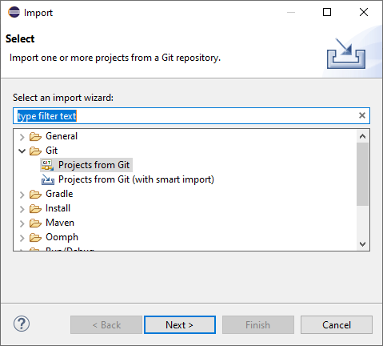
\includegraphics[]{images/EclipseImport}
\else
   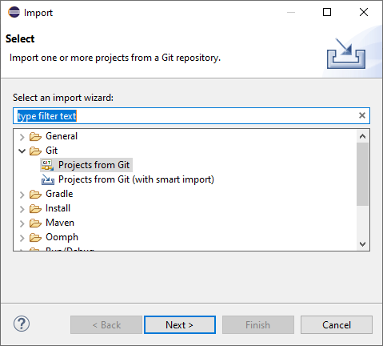
\includegraphics[width=0.55\textwidth]{images/EclipseImport}
\fi
\end{center}
%\caption{Eclipse Import dialog.}
%\label{EclipseImport:fig}
%\end{figure}

\item In the next dialog, choose {\sf Clone URI}, and click {\sf Next}.

\item A {\sf Source Git Repository} dialog will appear, as shown
below.
%in Figure \ref{SourceGitRepoDialog:fig}.
In the {\sf URI} field at the top, enter\\{\tt
https://github.com/artisynth/artisynth\_core.git}\\This will
automatically fill the {\sf Host} and {\sf Repository path} fields.
Click {\sf Next}.

%\begin{figure}[ht]
\begin{center}
\iflatexml
   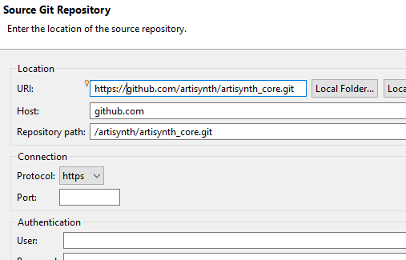
\includegraphics[]{images/EclipseGitRepoDialog}
\else
   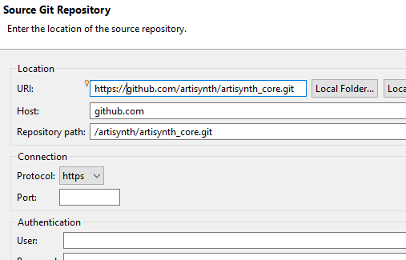
\includegraphics[width=0.55\textwidth]{images/EclipseGitRepoDialog}
\fi
\end{center}
%\caption{Eclipse Source Git Repository dialog.}
%\label{SourceGitRepoDialog:fig}
%\end{figure}

\item A {\sf Branch Selection} dialog will appear; uncheck {\tt svn}, so
that only {\tt master} is selected. Click {\sf Next}. 

\item A {\sf Local Destination} dialog will appear as shown
below,
% in (Figure \ref{LocalDestinationDialog:fig}), 
indicating the \directory{}
into which ArtiSynth will be placed locally. Use the default location,
or edit it to the desired location.  This will be your {\it ArtiSynth
home} \directory{}, and will be referred to later in this document as
{\tt <ARTISYNTH\_HOME>}. Click {\sf Next}.

%\begin{figure}[ht]
\begin{center}
\iflatexml
  \ifWindows
     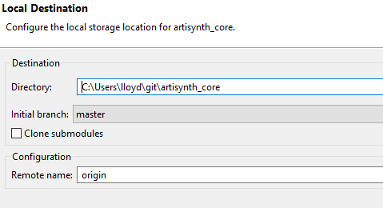
\includegraphics[]{images/LocalDestination}
  \else
     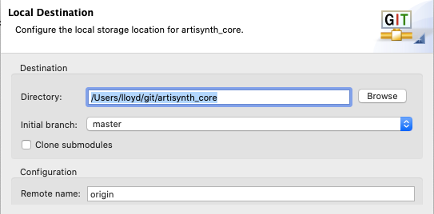
\includegraphics[]{images/LocalDestinationMacOS}
  \fi
\else
  \ifWindows
     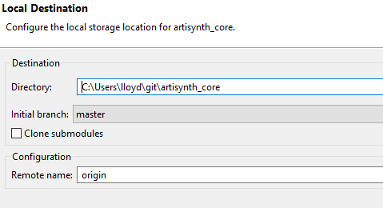
\includegraphics[width=0.55\textwidth]{images/LocalDestination}
  \else
     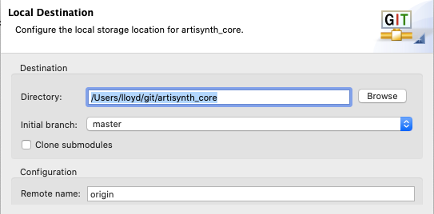
\includegraphics[width=0.55\textwidth]{images/LocalDestinationMacOS}
  \fi
\fi
\end{center}
%\caption{Eclipse Local Destination dialog.}
%\label{LocalDestinationDialog:fig}
%\end{figure}

\item ArtiSynth will now be downloaded; this may take a few minutes,
depending on your network connection speed. Another dialog will
appear, asking you to select to project import wizard.  Leave the
default (``{\sf Import existing Eclipse projects}'') selected, and
click {\sf Next}.

\item An {\sf Import Projects} dialog will appear, confirming that you
want to import {\tt artisynth\_core}. Leave everything as is, and
click {\sf Finish}.

\end{enumerate}

%\iflatexml\else
%\pagebreak
%\fi

{\tt artisynth\_core} has now been imported into Eclipse as a
project. However, we are not quite done. Eclipse will try to compile
{\tt artisynth\_core}, but will fail because some Java and native
libraries are missing. (These libraries are not included in the GitHub
repository because they are quite large.) The compile failure will be
indicated by a red exclamation mark to the left of the {\tt
artisynth\_core} project entry in the Package Explorer:
\begin{center}
\iflatexml
   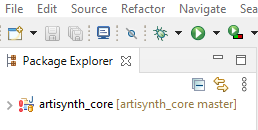
\includegraphics[]{images/artisynthBuildError}
\else
   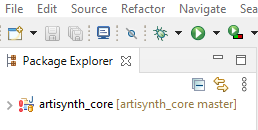
\includegraphics[width=0.35\textwidth]{images/artisynthBuildError}
\fi
\end{center}

The Java and native libraries must be downloaded separately, {\it
outside} of Eclipse.  
\ifWindows
Open a file explorer, navigate to the {\tt
<ARTISYNTH\_HOME>} \directory{} (described above), open the {\tt bin}
\directory{}, and click on the {\tt updateArtisynthLibs} batch file
(Figure \ref{UpdateArtisynthLibs:fig}).
This will load the libraries, temporarily displaying a terminal window
while doing so.
\else
Open a terminal window, change directories to {\tt <ARTISYNTH\_HOME>},
and run the command {\tt bin/updateArtisynthLibs}:
\begin{verbatim}
 > cd /path/to/ARTISYNTH_HOME
 > bin/updateArtisynthLibs
\end{verbatim}
\fi
The process may take a few minutes, depending on network speed.

\ifWindows
\begin{figure}[h]
\begin{center}
\iflatexml
   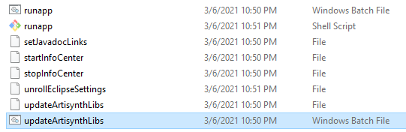
\includegraphics[]{images/UpdateArtisynthLibs}
\else
   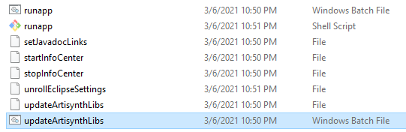
\includegraphics[width=0.6\textwidth]{images/UpdateArtisynthLibs}
\fi
\end{center}
\caption{%
{\tt updateArtisynthLibs} batch file in {\tt <ARTISYNTH\_HOME>\SEP bin}.}
\label{UpdateArtisynthLibs:fig}
\end{figure}
\fi

When the libraries are loaded, return to Eclipse, click on the {\tt
artisynth\_core} project to select it, then ``refresh'', either by
right clicking and selecting {\sf Refresh}, or by hitting the {\sf F5}
key. Eclipse should now find the libraries and compile ArtiSynth; a
green progress bar will appear at the lower right while compilation is
in progress.

After compilation is complete, ArtiSynth can be run by simply choosing
{\sf Run > Run} from the main menu. This works by invoking a
predefined {\it launch configuration} named ArtiSynth.  In some cases,
one may wish to adjust this launch configuration to set environment
variables, command line arguments, or Java JVM arguments that affect
how ArtiSynth behaves.  Instructions for doing so are contained in
Sections
\ref{EclipseEnvironmentVariables} and \ref{EclipseCommandArguments}.

\ifLinux
It is also possible to run ArtiSynth from a terminal window,
as described in Section \ref{artisynthCommandLine}.
\else % not Linux
It is also possible to run ArtiSynth from either a file browser or a
terminal window, as described in Sections \ref{runningFileBrowser}
and \ref{artisynthCommandLine}, respectively.
\fi
Detail on how to load and run demo models are given in
Section \ref{Running}.

\ifWindows
\subsection{Installation using Git for Windows}
\label{GitForWindows}

Git for Windows is an application that provides the user with a
terminal window interface that can be used for entering Git commands.
Users can choose between {\tt GitBash}, which provides a Unix-like
{\tt bash} shell, or {\tt GitCMD}, which provides a Windows {\tt CMD}
shell. {\tt GitBash} has several advantages, such as allowing users
to easily set environment variables in a {\tt .bashrc} file
(Section \ref{GitBashEnvironmentSettings}), and supplying a number of
Unix-like commands that can be convenient for tasks other than those
involving Git.

At the time of this writing, Git for Windows can be installed from
\href{https://git-scm.com/download/win}{git-scm.com/download/win}.

Once installed, ArtiSynth can then be installed and compiled by
opening a {\tt GitBash} window and entering the following commands
(where the `{\tt \$}' character indicates the {\tt GitBash} prompt
and should not be entered):
%
\begin{lstlisting}[]
 $ cd /path/to/install
 $ git clone https://github.com/artisynth/artisynth_core
 $ cd artisynth_core
 $ bin/updateArtisynthLibs
 $ make
\end{lstlisting}
%
The first line simply sets the current folder to the one under which
you wish to install ArtiSynth, as indicated by {\tt /path/to/install}.
(Note that {\tt GitBash} follows the Unix convention of using forward
slash ('/') instead of backslash ('\BKS ') to separate files.)  The
{\tt git clone} command then downloads ArtiSynth and extracts it to a
folder named {\tt artisynth\_core}, so that the ArtiSynth installation
directory (or {\tt <ARTISYNTH\_HOME>}) is\pdfbreak 
{\tt /path/to/install/artisynth\_core}. The {\tt updateArtisynthLibs}
command fetches additional libraries that are not included in the
GitHub repository for space reasons, and the {\tt make} command on the
last line is a Unix build utility provided by {\tt GitBash}; in this
situation, it compiles all the {\tt .java} files under {\tt
artisynth\_core}.

Once built, ArtiSynth can then be run (from within {\tt
artisynth\_core}) using the command
%
\begin{lstlisting}[]
  $ bin/artisynth
\end{lstlisting}
%
\begin{sideblock}
For convenience, if you place \ArtHome[\SEP bin] in your \PATH{}
environment variable (Section \ref{SettingPath}), 
then ArtiSynth can be run independently of the current
directory using the simple command
\begin{verbatim}
 % artisynth
\end{verbatim}
\end{sideblock}

ArtiSynth can also be installed and compiled using {\tt GitCMD},
with an analogous command sequence:
%
\begin{lstlisting}[]
 > cd \path\to\install
 > git clone https://github.com/artisynth/artisynth_core
 > cd artisynth_core
 > bin\updateArtisynthLibs
 > bin\compile
\end{lstlisting}
%
The only real difference is using backslash ('\BKS ') instead of
forward slash ('/') as a file separator, and the use of {\tt bin\BKS
compile} instead of {\tt make} (which is not supported in {\tt Git
CMD}). {\tt compile} is a command supplied by ArtiSynth that compiles
all {\tt .java} files located under the current folder.
\else % not Windows
\subsection{Installation using the command line}

If your \SYSTEM{} distribution has Git installed, then you can
install ArtiSynth from a terminal window using the following
commands:
%
\begin{lstlisting}[]
 > cd /path/to/install
 > git clone https://github.com/artisynth/artisynth_core
 > cd artisynth_core
 > bin/updateArtisynthLibs
\end{lstlisting}
%
The first line simply sets the current folder to the one under which
you wish to install ArtiSynth, as indicated by {\tt /path/to/install}.
The {\tt git clone} command then downloads ArtiSynth and extracts it
to a folder named {\tt artisynth\_core}, so that the ArtiSynth
installation directory (or {\tt <ARTISYNTH\_HOME>}) is {\tt
/path/to/install/artisynth\_core}. The {\tt updateArtisynthLibs}
command fetches additional libraries that are not included in the
GitHub repository for space reasons.
\ifMacOS

If your system has {\tt make} installed (usually via XCode or
an equivalent), you can then compile ArtiSynth by simply entering
the command 
%
\begin{lstlisting}[]
 > make
\end{lstlisting}
%
from within {\tt artisynth\_core}. {\tt make} is a Unix build utility
which in this situation compiles all the {\tt .java} files under {\tt
artisynth\_core}. If you don't have {\tt make}, you can do
the following instead:
%
\begin{lstlisting}[]
 > bin/compile
\end{lstlisting}
%
{\tt compile} is an ArtiSynth command line utility that compiles all {\tt .java}
files located under the current folder.
\fi % end MacOS
\ifLinux

ArtiSynth can then be compiled using the command
%
\begin{lstlisting}[]
 > make
\end{lstlisting}
%
within the {\tt artisynth\_core} directory.
\fi % end Linux

Once compiled, ArtiSynth can be run from the command line as described
in Section \ref{artisynthCommandLine}.
\ifMacOS
It can also be run from a file browser, as described
in Section \ref{runningFileBrowser}.
\fi
%
\fi % end not windows

Details on how to load and run demo models are given in
Section \ref{Running}.

Note that once you have installed ArtiSynth, you still have the option
to later import it into an IDE such as Eclipse. For Eclipse
specifically, this is done by importing it as an {\it external
project}, as described in Section \ref{importingExternalProjects}.

\section{Loading and Running Models}
\label{Running}

After ArtiSynth starts up, you can load and run demonstration
models. Do this by selecting {\sf Models > Demos} from the main menu
and choosing a demo model (Figure \ref{ModelSelectionMenu:fig}).

\begin{figure}[ht]
\begin{center}
\iflatexml
   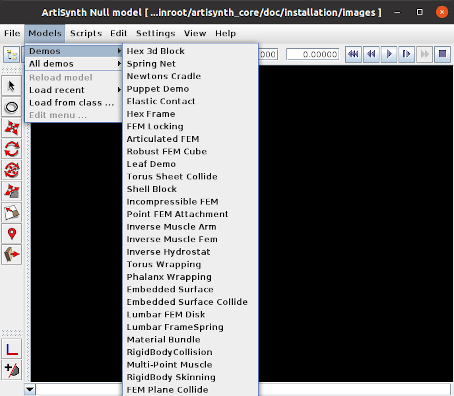
\includegraphics[]{images/ArtiSynthDemoMenu}
\else
   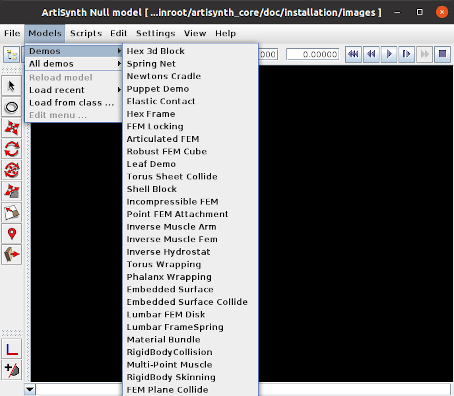
\includegraphics[width=0.65\textwidth]{images/ArtiSynthDemoMenu}
\fi
\end{center}
\caption{The ArtiSynth model selection menu.}
\label{ModelSelectionMenu:fig}
\end{figure}

\iflatexml\else\pagebreak\fi

\ifMacOS
\begin{sideblock}
On older versions of {\tt MacOS}, errors similar to the following
may appear on the Eclipse Console output:
\begin{verbatim}
 2021-03-12 11:01:16.949 java[585:230b] invalid drawable 
\end{verbatim}
This is due to a problem in the default version of the Java-OpenGL
(JOGL) interface. To fix it, go back to the terminal window, and
from the ArtiSynth home directory run the command
\begin{verbatim}
 > bin/installJOGL2.3.2
\end{verbatim}
Then recompile ArtiSynth.
\end{sideblock}
\fi

Once a model is loaded, it will appear in the viewer, and simulation
can be controlled using the ``play'' controls located at the upper right
of the application window:

\begin{center}
\iflatexml
  
\includegraphics[]{../uiguide/images/playControls}
\else
  
\includegraphics[width=2.5in]{../uiguide/images/playControls}
\fi
\end{center}

From left to right, these are: step size control, which controls the
simulation step size (in seconds); current simulation time (in
seconds); and the {\sf reset}, {\sf skip-back}, {\sf play/pause}, {\sf
single-step}, {\sf skip-forward} and {\sf stop-all} buttons.  Starting
and stopping a simulation is done by clicking {\sf play/pause}, while
{\sf reset} resets the simulation to time 0.  The {\sf single-step}
button advances the simulation by one time step. The {\sf stop-all}
button will also stop the simulation, as well as any Jython commands
or scripts that are running.

\ifMacOS

\begin{sideblock}
On newer versions of {\tt MacOS}, another problem that may occur when
trying to run ArtiSynth models is that MacOS may complain about using
a nonvalidated external library. This will take the form of a console
error that looks like this:
\begin{verbatim}
 ...
 /Users/lloyd/git/artisynth_core/lib/MacOS64/libPardisoJNI.11.1.2.1.dylib)
 not valid for use in process using Library Validation: library load disallowed
 by system policy 
 ...
\end{verbatim}
The problem here is that one or more of the native libraries are not
``known'' to Apple and are therefore not trusted. General information
on working around this problem is described here:

\href{https://support.apple.com/en-ca/HT202491}{support.apple.com/en-ca/HT202491}

The short version is to immediately open your Security and Privacy
settings after the error occurs, and then, near the bottom of the {\sf
General} tab, you should see a notification about the blocked
application with a button to the right labeled {\sf Open
Anyway}. Clicking that button will grant the application a security
exception.
\end{sideblock}

\fi

Detailed information on how to use the ArtiSynth GUI for model
visualization, navigation and simulation control is given in the
\artisynthManual{uiguide}{ArtiSynth User Interface Guide}.

Figure \ref{SpringNetDemo:fig} shows ArtiSynth with the {\sf Spring
Net} demo loaded.

\begin{figure}[ht]
\begin{center}
\iflatexml
   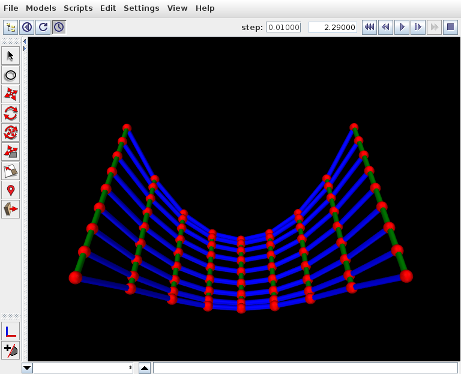
\includegraphics[]{images/SpringNetDemo}
\else
   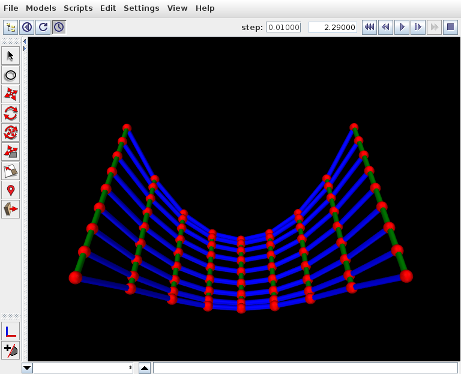
\includegraphics[width=0.60\textwidth]{images/SpringNetDemo}
\fi
\end{center}
\caption{ArtiSynth with the Spring Net demo loaded.}
\label{SpringNetDemo:fig}
\end{figure}

\subsection{Other ways to load models}

It is possible to load models in several ways:

\begin{itemize}

\item Using a model menu entry, as described above;

\item Specifying the Java class describing the model
({\sf ``Load from class ...''} from the {\sf Models} menu);

\item Specifying a {\tt .art} file containing a text
representation of the model ({\sf ``Load model ...''} from the {\sf
File} menu);

\item Reloading a recently loaded model 
({\sf ``Load recent''} from the {\sf Models} menu).

\end{itemize}

It is also possible to configure ArtiSynth to load a specific model
when it starts up; see ``Loading, Simulating and Saving Models'' in the
\artisynthManual{uiguide}{ArtiSynth User Interface Guide}.
The model menu can also be customized, as described in ``Customizing
the Model Menu''.

\subsection{Viewing and interacting with models}

The ArtiSynth user interface provides a variety of tools for exploring
and interacting with models, as described in depth in
the \artisynthManual{uiguide}{ArtiSynth User Interface Guide},
including:

\begin{itemize}

\item 3D viewers with grids and clipping planes;

\item Component selection using either a viewer or
a tree-based navigation panel;

\item Property inspection and editing for selected components;

\item 3D fixtures for translating, rotating and
applying forces to models and their components;

\item A timeline for viewing and organizing input/output data streams
known as {\it probes};

\item Some simple model editing, including the ability to interactively
delete components and add marker points;

\item Making movies from simulations.

\end{itemize}

\subsection{Command line arguments}
\label{CommandLineArguments}

If you are running ArtiSynth from a terminal window
(Section \ref{artisynthCommandLine})
\ifWindows
or {\tt GitBash} (Section \ref{GitForWindows})
\fi
then you can supply it with
command line arguments to control different aspects of its behavior.
A full list of these can be seen by running {\tt artisynth} with the {\tt
-help} option:
\begin{verbatim}
 > artisynth -help
\end{verbatim}
Descriptions of these options appear in various places within the
ArtiSynth documentation. For example, one commonly used option is
{\tt -model <modelClassName>}, which instructs ArtiSynth to preload a
model associated with a given class name:
\begin{verbatim}
 > artisynth -model artisynth.demos.mech.SpringMeshDemo
\end{verbatim}

If you are running under Eclipse, command line arguments can be set in
the launch configuration, as described in
Section \ref{EclipseCommandArguments}.

\section{Creating and Adding Models}
\label{AddingModels}

Most users will want to develop their own ArtiSynth models using Java
code. This is done by creating a special Java {\it model} class, which
is a subclass of
\javaclass[artisynth.core.workspace]{RootModel} and which contains a
{\tt build()} method that assembles the model from the various Java
components that ArtiSynth provides. For example, suppose your model
class is called {\tt MyModel}. This will be implemented inside a Java
source file called {\tt MyModel.java}, a skeleton implementation of
which might look like this:
%
\lstset{commentstyle=\color{mygreen}}
\begin{lstlisting}[]
package artisynth.models.mymodels;

// import statements to access classes:
import maspack.matrix.*;                  // vectors and matrices
import artisynth.core.mechmodels.*;       // mechanical models and components
import artisynth.core.workspace.RootModel;

// model class definition:
public class MyModel extends RootModel {

   public void build (String[] args) {
      // ... model is assembled here ...
   }
}
\end{lstlisting}
\lstset{commentstyle=\color{myblack}}
%
Full details on how to create a model in Java and the components that
are available to do so are given in
the\pdfbreak
\artisynthManual{modelguide}{ArtiSynth Modeling Guide}. For this
discussion, we will consider only how to add a model to ArtiSynth once
it has been created. The easiest way to do this is to add its source
code to the ArtiSynth source code, as described below. However, as
a general practice, it is recommended that the model source code
be kept separate from ArtiSynth, as described in
Section \ref{IntegratingExternalModels}.

\subsection{Model packages}

A model should be implemented inside a Java {\it package}, which will
contain the model class, and perhaps other supporting classes used to
implement it. The package is defined by the {\tt package} statement at
the beginning of each {\tt .java} file. For the {\tt MyModel} example
above, the package is {\tt artisynth.models.mymodels}.

Java enforces certain rules for how its source code is organized.  In
particular, all the {\tt .java} files associated with a specific
package must be placed in the same folder, which in turn must be located in a
\directory{} tree that reflects the package hierarchy. For
example, source code for the package {\tt pack.foo.bar} must be placed
in a folder whose path (relative to the top of the source tree) is
{\tt pack\SEP foo\SEP bar}.  For the {\tt MyModel} example, {\tt
MyModel.java} must be placed in
a folder {\tt artisynth\SEP models\SEP mymodels} relative to the top
of the source tree.

The source code tree for ArtiSynth is rooted at {\tt
<ARTISYNTH\_HOME>\SEP src}. It already contains a large number of
model classes located in packages such as {\tt
artisynth.demo.mech}, whose source code is therefore located at

{\tt <ARTISYNTH\_HOME>\SEP src\SEP artisynth\SEP demos\SEP mech}

The easiest way to add your own model to ArtiSynth is to simply add
the source code for its package to the appropriate location under {\tt
<ARTISYNTH\_HOME>\SEP src}. For {\tt MyModel}, the source code would
therefore be placed in

{\tt <ARTISYNTH\_HOME>\SEP src\SEP artisynth\SEP models\SEP mymodels}

Since the ArtiSynth source tree already contains the (empty) folder
{\tt artisynth\SEP models}, in this case it would only be necessary to
add the {\tt mymodels} folder below it.

\begin{sideblock}
Multiple models may be placed in any given package. For example, {\tt
artisynth.demos.tutorial} contains a large number of models used as
examples for the Modeling Guide.
\end{sideblock}

\subsection{Compiling models}

When source code is added or modified within the ArtiSynth source
tree, it needs to be compiled. How this is done depends on your
development environment.

If you are using Eclipse and automatic building is enabled for a
project (such as {\tt artisynth\_core}), compilation will occur
automatically whenever that project's {\tt .java} files are
modified. To see if automatic building is enabled, select the project
in the Package Explorer, open the {\sf Project} menu and check {\sf
Build Automatically}. If automatic building is not enabled, the
project can be built by selecting {\sf Build Project}.

\begin{sideblock}
If you add or edit source files from {\it outside} Eclipse, for
example by using an external text editor, then you need to {\it
refresh} the project in order for Eclipse to notice the changes.  To
refresh, select the project in the Package Explorer, and then either
right-click and choose {\sf Refresh}, or simply hit the {\sf F5} key.
\end{sideblock}

If you are compiling from the command line 
\ifWindows
or {\tt GitBash}%
\fi
, using either the {\tt make} or {\tt compile} commands described
earlier, then running these in any given source \directory{}
will compile all the {\tt .java} files contained below it. This will
typically be faster than compiling the entire source tree by running
{\tt make} or {\tt compile} from {\tt <ARTISYNTH\_HOME>}.

\begin{sideblock}
To be able to run {\tt compile} from any \directory{},
place \ArtHome[\SEP bin] in your \PATH{} environment variable
(Section \ref{SettingPath}).
\end{sideblock}

\begin{sideblock}
If you add a {\it new} package \directory{} and want to run {\tt make}
from that \directory{}, you will need to add a {\tt Makefile} to
it. The easiest way to do this is to simply copy an existing {\tt
Makefile} from another package and adjust the {\tt PACKAGE\_NAME} and
{\tt ROOT\_DIR} entries; the number of `{\tt ..}'  entries in {\tt
ROOT\_DIR} should equal the number of ``up'' steps needed to reach
{\tt <ARTISYNTH\_HOME>}.
\end{sideblock}

\subsection{Finding models in the model menu}

Once a model has been added to ArtiSynth, it is useful to be able to
run it directly from the {\it model menu}, located under {\sf Models}
in the main menu bar.

By default, the model menu locates all models in the packages
(and subpackages) of {\tt artisynth.demos} and\pdfbreak {\tt
artisynth.model}, and makes then available under the entries {\sf All
demos >} and {\sf All models >}, respectively. Therefore, if your
model is located in one of these packages, it will automatically
appear in the {\sf Models} menu. If your model is located in a
different package, you can load it either by directly specifying its
class path, or by customizing the {\sf Models} menu.  These options
are described in the sections ``Loading by class path'' and
``Customizing the Model Menu'' of the
\artisynthManual{uiguide}{ArtiSynth User Interface Guide},

\section{Settings and the user configuration folder}
\label{UserConfigFolder:sec}

When ArtiSynth is first run, it creates a configuration folder named
{\tt ArtiSynthConfig} beneath the user's home folder. Various
subfolders within this are used to store startup settings, model menu
customizations, etc.

Startup settings that can be configured include those for the viewer,
mouse bindings, model interaction and simulation, as discussed in the
``Preferences'' section and elsewhere in the
\artisynthManual{uiguide}{ArtiSynth User Interface Guide}.

\section{Integrating external models}
\label{IntegratingExternalModels}

While it is easiest to add a model to ArtiSynth by simply placing its
source code under {\tt <ARTISYNTH\_HOME>\SEP src}, as described in
Section \ref{AddingModels}, it is usually best practice to keep model
source code separate from ArtiSynth. This is largely to avoid
conflicts when ArtiSynth is updated (Section \ref{UpdatingArtiSynth})
or reinstalled.

When model source code is external to ArtiSynth, one must manage two
things:

\begin{enumerate}

\item Making the ArtiSynth classes visible to the Java compiler
when compiling the code;

\item Making the model classes visible to ArtiSynth when running
the model.

\end{enumerate}

This involves managing the class path used by either the Java compiler
or by ArtiSynth.

For purposes of this discussion, we will assume that the model is
contained under a top-level \directory{} denoted by {\tt <MYPROJECT>},
and that the root \directories{} for the Java source code and class
files are {\tt <MYPROJECT>\SEP src} and
\pdfbreak
{\tt <MYPROJECT>\SEP classes}, respectively. This Java file structure
is common, and is used by {\tt artisynth\_core} and most other
projects currently associated with ArtiSynth.

\subsection{Making ArtiSynth visible to the compiler}

How this is done depends on your development environment.

\subsection{Eclipse development}

When using Eclipse, the project will also be associated with an
Eclipse project name, which we will call {\tt myproject}.  In order
for {\tt myproject} to compile, the ArtiSynth project {\tt
artisynth\_core} should be added to the {\it build path} of {\tt
myproject}, as described in
Section \ref{AddingProjectsToBuildPath}. This will ensure that the
ArtiSynth classes are added to the class path used by the Java
compiler.

\begin{sideblock}
Some projects, such as {\tt artisynth\_models}, already have their
build path preconfigured to contain {\tt artisynth\_core}, and so for
them this step is unnecessary.
\end{sideblock}

\subsection{Command line development}
\label{CommandLineDevel}

If you are compiling from the command line 
\ifWindows
or {\tt GitBash}%
\fi
, then the {\tt compile} command described earlier will still work,
provided that, as assumed above, {\tt <MYPROJECT>} contains the source
and classes \directories{} {\tt src\SEP} and {\tt classes\SEP}. The
{\tt compile} command will supply the Java compiler with a class path
containing all the ArtiSynth classes, plus {\tt <MYPROJECT>\SEP
classes}. If {\it additional} classes are needed (such as external
JAR files or class \directories{} from other projects), they
may be added by setting them in the {\tt CLASSPATH} environment
variable (Section \ref{EnvironmentVariables}).

Use of the {\tt make} command will require setting up {\tt Makefile}s
in the \directories{} in which you wish to run {\tt make}. It will
also (usually) require setting the {\tt CLASSPATH} environment
variable to contain the ArtiSynth
class path entries,
\ifWindows
\begin{verbatim}
<ARTISYNTH_HOME>\classes;<ARTISYNTH_HOME>\lib\*
\end{verbatim}
\else
\begin{verbatim}
<ARTISYNTH_HOME>/classes;<ARTISYNTH_HOME>/lib/*
\end{verbatim}
\fi
where as usual {\tt <ARTISYNTH\_HOME>} should be expanded to the path
for the ArtiSynth installation directory.  The character `{\tt *}'
functions as a wildcard to specify all the JAR files in
{\tt <ARTISYNTH\_HOME>\SEP lib}.

\subsection{Making external models visible to ArtiSynth}
\label{MakingExternalModelsVisible}

\subsection{Running from Eclipse}

When running ArtiSynth under Eclipse, you can make {\tt myproject}'s
models visible by adding {\tt myproject} to the ArtiSynth launch
configuration, as described in Section
\ref{AddingProjectsToLaunch}. 

\subsection{Using the external classpath}
\label{ExternalClasspath:sec}

External models can be made visible to ArtiSynth by adding any needed
class \directories{} and JAR files to the {\it external class path}.
The easiest way to do this is to select ``{\sf Settings > External
classpath ...}'' from the {\sf Settings} menu, which will open an
external classpath editor as shown in
Figure \ref{externalClasspathEditor:fig}, allowing the necessary
class \directories{} and JAR files to be added.  The classpath entries
are displayed in a large panel on the left (which will initially be
blank after ArtiSynth is first installed).  

\begin{figure}[h]
\begin{center}
\iflatexml
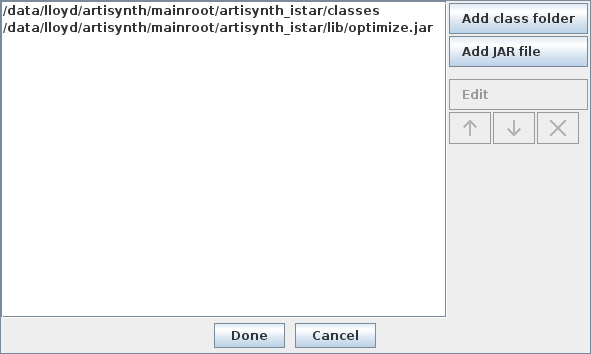
\includegraphics[]{images/externalClasspathEditor}
\else
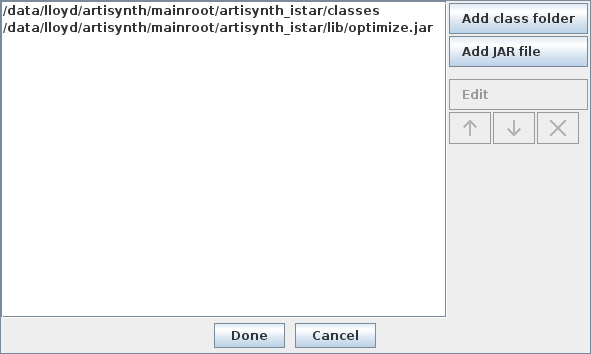
\includegraphics[width=5in]{images/externalClasspathEditor}
\fi
\end{center}
\caption{The external classpath editor.}%
\label{externalClasspathEditor:fig}
\end{figure}

As an example, assume that
the model class files are contained under {\tt <MYPROJECT>\SEP
classes}, and that the JAR file {\tt <MYPROJECT>\SEP lib\SEP
dicom.jar} is also required.  If {\tt <MYPROJECT>} is located
at \ifWindows {\tt C:\SEP research\SEP myproject}%
\else {\tt /research/myproject}%
\fi , then the following entries should be added to
the external classpath:
\ifWindows
\begin{verbatim}
C:\research\myproject\classes
C:\research\myproject\lib\dicom.jar
\end{verbatim}
\else % not Windows
\begin{verbatim}
/research/myproject/classes
/research/myproject/lib/dicom.jar
\end{verbatim}
\fi % end not Windows

\begin{sideblock}
ArtiSynth must be restarted for external classpath changes to come
into effect.
\end{sideblock}

More details are given in the section ``Setting the external classpath''
of the 
\artisynthManual{uiguide}{ArtiSynth User Interface Guide}.
The external classpath is stored in the file {\tt EXTCLASSPATH}
in the user configuration folder and can be edited directly
(Section \ref{EXTCLASSPATHFile}).

The external classpath can be used when running from Eclipse or any
other IDE.

\subsection{Setting the CLASSPATH environment variable}
\label{SettingCLASSPATH}

When running ArtiSynth from the command line, external models can also
be made visible by adding class folders and JAR files to the {\tt
CLASSPATH} environment variable, as described in
Section \ref{EnvironmentVariables}. For the example of
Section \ref{ExternalClasspath:sec}, we could instead add the following to
{\tt CLASSPATH}:
\ifWindows
\begin{verbatim}
   C:\research\myproject\classes;C:\research\myproject\lib\dicom.jar
\end{verbatim}
\else
\begin{verbatim}
   /research/myproject/classes;/research/myproject/lib/dicom.jar
\end{verbatim}
\fi
Note that in this situation the ArtiSynth class files {\it do not}
need to be included in {\tt CLASSPATH}, as they will be added
automatically.

\subsection{Using the {\tt -cp} option}

ArtiSynth also provides the command line option {\tt -cp} which allows
a class path to be specified directly:
\ifWindows
\begin{verbatim}
   > artisynth -cp "C:\research\myproject\classes;C:\research\myproject\lib\dicom.jar"
\end{verbatim}
\else
\begin{verbatim}
   > artisynth -cp "/research/myproject/classes:/research/myproject/lib/dicom.jar"
\end{verbatim}
\fi
Class paths specified using {\tt -cp} will {\it replace} any specified
through the {\tt CLASSPATH} variable.

\section{Installing {\tt artisynth\_models}}
\label{ArtiSynthModels}

{\tt artisynth\_models} is an open source collection of anatomical
models, focused primarily on the head and neck region
(see \href{https://www.artisynth.org/models}{www.artisynth.org/models}).
It can be obtained either as a precompiled release, or from GitHub.

Once installed, the models will appear in the ArtiSynth {\sf Models}
menu under {\sf Models >} and {\sf All models >}.

\subsection{Installing a precompiled release}

If you are running a precompiled release of ArtiSynth,
then you will need to use the corresponding precompiled release
of {\tt artisynth\_models}, which can be 
obtained from
\begin{verbatim}
  www.artisynth.org/Software/ModelsDownload
\end{verbatim}
Download the distribution you want and unzip it in your desired location;
the recommended spot is right next to {\tt artisynth\_core}.

{\tt artisynth\_models} comes preconfigured with Eclipse project
files, and so can be immediately imported into Eclipse as an external
project, as described in Section \ref{importingExternalProjects}.  To
make the models visible to ArtiSynth when running from Eclipse, it
will be necessary to add {\tt artisynth\_models} to the ArtiSynth
launch configuration, as described in Section
\ref{AddingProjectsToLaunch}.

If you are running ArtiSynth from the command line
\ifWindows
or the {\tt artisynth.bat} file%
\fi
, you will need to ensure that the class \directory{} {\tt
artisynth\_models\SEP classes} is visible to ArtiSynth, as described
in Section \ref{MakingExternalModelsVisible}.

\subsection{Installing from GitHub}

The latest development version of {\tt artisynth\_models} is available
from GitHub at the URL
\begin{verbatim}
   https://github.com/artisynth/artisynth_models.git
\end{verbatim}

\subsubsection{Installation using Eclipse}

If you are using Eclipse, you can install {\tt artisynth\_models} in
the same way as for {\tt artisynth\_core} (Section
\ref{EclipseInstallation}):

\begin{enumerate}

\item Select {\sf ``File > Import ...''}, open
{\sf ``Git > Projects from Git''} in the Import dialog,
and click {\sf Next}.

\item In the {\sf Select Repository Source}
dialog, choose {\sf Clone URI}, and click {\sf Next}.

\item In the {\sf Source Git Repository} dialog,
enter\\
{\tt https://github.com/artisynth/artisynth\_models.git}\\
in the {\sf URI} field at the top, and click {\sf Next}.

\item In the {\sf Branch Selection} dialog, uncheck {\tt svn}
and click {\sf Next}.

\item In the {\sf Local Destination} dialog,
adjust the install location if desired, and click {\sf Next}.

\item {\tt artisynth\_models} will now be downloaded.
A ``wizard'' dialog will
then appear. Leave the default ({\sf ``Import existing Eclipse
projects''}) selected, and click {\sf Next}.

\item In the {\sf Import Projects} dialog, click {\sf Finish}.

\end{enumerate}

{\tt artisynth\_models} should now compile automatically; there is no
need to download external libraries. However, to 
make the models visible to ArtiSynth when running from Eclipse, it
will be necessary to add {\tt artisynth\_models} to the ArtiSynth
launch configuration, as described in Section
\ref{AddingProjectsToLaunch}.

\ifWindows
\subsubsection{Installation using Git for Windows}

If you have Git for Windows installed (Section \ref{GitForWindows}),
{\it and} you have placed {\tt <ARTISYNTH\_HOME>\SEP bin} in your {\tt
Path} environment variable (Section \ref{SettingPath}), allowing
the {\tt compile} command to be called from any folder, then {\tt
artisynth\_models} can be installed from {\tt GitBash} as follows:
%
\begin{lstlisting}[]
 $ cd /path/to/install
 $ git clone https://github.com/artisynth/artisynth_models
 $ cd artisynth_models
 $ compile
\end{lstlisting}
%
\else
\subsubsection{Installation from the command line}
If you have placed {\tt <ARTISYNTH\_HOME>\SEP bin} in your \PATH{}
environment variable (Section \ref{SettingPath}), so that the
{\tt compile} command can be called from any \directory{}, then {\tt
artisynth\_models} can be installed from a terminal window as follows:
%
\begin{lstlisting}[]
 > cd /path/to/install
 > git clone https://github.com/artisynth/artisynth_models
 > cd artisynth_models
 > compile
\end{lstlisting}
%
\fi
The last line uses the {\tt compile} command instead of {\tt make}
because the latter will not work unless the {\tt CLASSPATH}
environment variable has been set to include the ArtiSynth class path
entries, as described in Section \ref{CommandLineDevel}.

If you run ArtiSynth from the command line, you will need to ensure
that {\tt artisynth\_models\SEP classes} is visible to ArtiSynth, as
described in Section \ref{MakingExternalModelsVisible}.

\section{Updating ArtiSynth}
\label{UpdatingArtiSynth}

One reason to install ArtiSynth from GitHub is to be able to update
the codebase to incorporate new features and bug fixes.  When a
significant update occurs, a posting is made to the ArtiSynth update
log, currently located at
\artisynthManual{updates}{www.artisynth.org/doc/html/updates/updates.html}.
Users may also be notified via the {\tt artisynth-updates} email list.

Eclipse users may update simply by selecting the {\tt artisynth\_core}
in the {\sf Package Explorer} and then right clicking and choosing
{\sf Team > Pull}.

\ifWindows
If Git for Windows is installed (Section \ref{GitForWindows}),
then updating may be done using {\tt GitBash}:
\begin{verbatim}
 $ cd <ARTISYNTH_HOME>
 $ git pull
\end{verbatim}
\else % not Windows 
Updating may also be done from a terminal window: 
\begin{verbatim}
 > cd <ARTISYNTH_HOME>
 > git pull
\end{verbatim}
\fi % end not Windows

\begin{sideblock}
If local changes have been made to {\tt artisynth\_core} that
interfere with the changes made by the update, a Git pull operation
may result in a {\it conflict}.  Conflict resolution is outside the
scope of this document, but documentation on this is available online.
Conflicts should not occur if local changes have not been made to {\tt
artisynth\_core}.
\end{sideblock}

Other Git-based projects, such as {\tt artisynth\_models}, may be
updated similarly.

\subsection{Library updates}

Occasionally, a software update will be accompanied by a change in the
libraries located in \ArtHome[\SEP libs].  When this happens, it will
be indicated on the ArtiSynth update log and appropriate instructions
will be given. In these cases, one should also update the ArtiSynth
libraries. 

The easiest way to do this is from within ArtiSynth, by selecting
{\sf ``Update Libraries''} at the bottom of the {\sf File} menu.

Libraries can
also be updated using the command {\tt updateArtisynthLibs} located in
{\tt <ARTISYNTH\_HOME>\SEP bin}. This can be done from a terminal
window:
\ifWindows
\begin{verbatim}
 > cd <ARTISYNTH_HOME>
 > bin\updateArtisyntnLibs
\end{verbatim}
It can also be done from a file browser, by navigating
to {\tt <ARTISYNTH\_HOME>} and clicking on {\tt updateArtisynthLibs.bat}.
(Figure \ref{UpdateArtisynthLibs:fig}).
\else
\begin{verbatim}
 > cd <ARTISYNTH_HOME>
 > bin/updateArtisynthLibs
\end{verbatim}
\fi

\section{The Eclipse IDE}
\label{EclipseIDE}

Eclipse is an integrated development environment (IDE) commonly used
for Java code development, and many ArtiSynth developers use it for
both developing models in Java and for running the system. This
section describes how to install Eclipse and provides some other
information relevant to ArtiSynth users.  A general introduction to
Eclipse is beyond the scope of this document, but there are many
Eclipse resources available online.

\subsection{Installing Eclipse}
\label{InstallingEclipse}

This document describes specifically the installation of Eclipse
2020-12; other versions should be similar.

Eclipse can be downloaded from
\href{https://www.eclipse.org/downloads/packages}%
{www.eclipse.org/downloads/packages}. From this page, choose ``{\sf
Eclipse IDE for Java Developers}'',
\ifWindows
{\sf Windows x86\_64}, which will download the file
\begin{verbatim}
  eclipse-java-2020-12-R-win32-x86_64.zip
\end{verbatim}
Unzip this into a convenient \directory{}, such as for example:
\begin{verbatim}
  C:\eclipse\eclipse-2020-12
\end{verbatim}
Open this \directory{} with a file explorer, and you will see the eclipse
application:

\begin{center}
   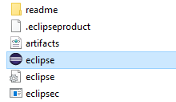
\includegraphics[width=0.25\textwidth]{images/EclipseApp}
\end{center}

Click on this to open it. 
\fi
\ifMacOS
{\sf macOS x86\_64}, which will download the file
\begin{verbatim}
  eclipse-java-2020-12-R-macosx-cocoa-x86_64.dmg
\end{verbatim}
Open this file, click on the ``Eclipse Installer'',
select ``Eclipse IDE for Java Developers'', and follow
the install instructions. When the install is complete,
click the {\sf Launch} button.
\fi
\ifLinux
{\sf Linux x86\_64}, which will download the file
\begin{verbatim}
  eclipse-java-2020-12-R-linux-gtk-x86_64.tar.gz
\end{verbatim}
Untar this file into any desired install location,
and then run the {\tt eclipse} executable in the
top-level directory.
\fi
A dialog will appear, asking you to select a workspace \directory{}
(Figure \ref{EclipseWorkspace:fig}).
This is where Eclipse settings and project information will be
stored. Unless you have a another Eclipse already installed, the
default location should be fine. (Remember also to check the ``{\sf
Use this as the default ...}''  box so that this query won't appear
every time you open Eclipse.) 
Next, click {\sf Launch}.  A welcome
page will appear; close this. A ``donate'' panel may also appear;
close this too.  You should then see an empty Eclipse display, similar
to Figure \ref{EmptyEclipse:fig}.

\begin{figure}[ht]
\begin{center}
\iflatexml
  \ifWindows
     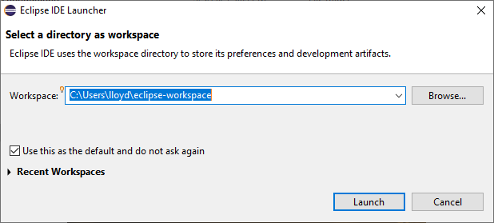
\includegraphics[]{images/EclipseWorkspaceDialog}
  \else
    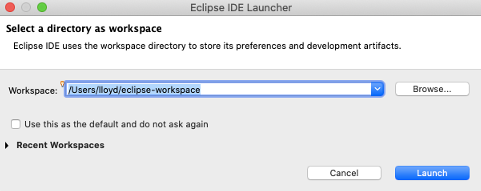
\includegraphics[]{images/EclipseWorkspaceDialogMacOS}
  \fi
\else
  \ifWindows
     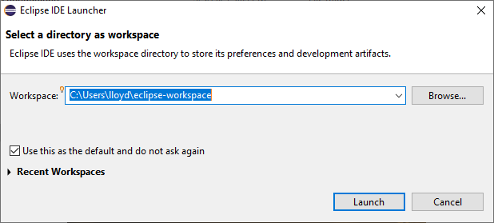
\includegraphics[width=0.7\textwidth]{images/EclipseWorkspaceDialog}
  \else
    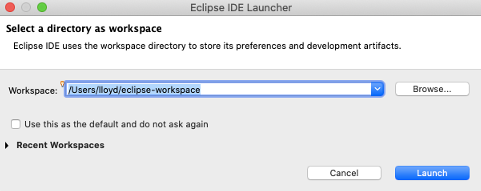
\includegraphics[width=0.7\textwidth]{images/EclipseWorkspaceDialogMacOS}
  \fi
\fi
\end{center}
\caption{Eclipse Workspace dialog.}
\label{EclipseWorkspace:fig}
\end{figure}
%
This is where Eclipse settings and project information will be
stored. Unless you have a another Eclipse already installed, the
default location should be fine. (Remember also to check the ``{\sf
Use this as the default ...}''  box so that this query won't appear
every time you open Eclipse.) 
Next, click {\sf Launch}.  A welcome
page will appear; close this. A ``donate'' panel may also appear;
close this too.  You should then see an Emily Eclipse display, similar
to Figure \ref{EmptyEclipse:fig}.

\begin{figure}[ht]
\begin{center}
\iflatexml
   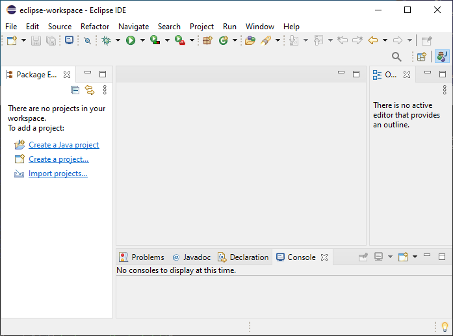
\includegraphics[]{images/EmptyEclipse}
\else
   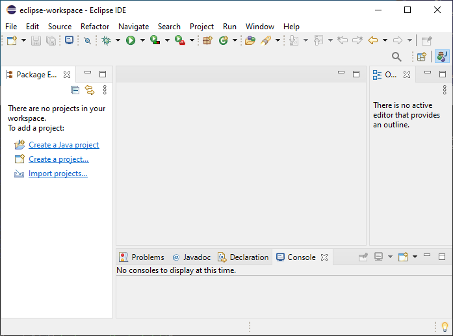
\includegraphics[width=0.7\textwidth]{images/EmptyEclipse}
\fi
\end{center}
\caption{An empty, newly initialized Eclipse console.}
\label{EmptyEclipse:fig}
\end{figure}

\ifMacOS
\begin{sideblock}
Before closing Eclipse, you may want to pin its icon to your dock
to make it easier to restart.
\end{sideblock}
\fi

\subsubsection{Setting Eclipse to use the correct Java JDK}
\label{EclipseJDK:sec}

Newer versions of Eclipse come with their own version of
Java. However, since we generally want to use our own Java JDK (such
as Java 8, as described in Section \ref{InstallingJava}), we need to
configure Eclipse to use that instead. This can be done as follows:

\begin{enumerate}

\item From the main menu, select 
\ifMacOS
``{\sf Eclipse > Preferences ...}''.
\else
``{\sf Window > Preferences}''.
\fi

\item A {\sf Preferences} dialog will open. In the left panel, select
``{\sf Java > Installed JREs}'', which will open an {\sf Installed JREs}
panel.
\ifMacOS % begin macOS
On MacOS, all installed JDKs {\it should} appear in the panel
(Figure \ref{InstalledJREs:fig}), including the Eclipse default and
the JDK which you want to use.  Click on the box to the left of
your JDK entry to select it; ignore warnings about Java 15
compatibility.
\else  % begin Not macOS
Click the {\sf Add...} button at the right.

\item A {\sf JRE Type} dialog will appear. Leave ``Standard VM''
selected in the dialog and click {\sf Next}.

\item A {\sf JRE Definition} dialog will appear. In the ``{\sf JRE home}''
field at the top, enter the installation \directory{} for your JDK.
\ifWindows % begin Windows
On Windows, this is likely to be a location like {\tt C:\BKS Program
Files\BKS Java\BKS jdk1.8.0\_281}. Specifying the java
home \directory{} will cause some other fields to fill in
automatically, as seen in Figure \ref{JREDefinition:fig}.
%
\begin{figure}[ht]
\begin{center}
\iflatexml
   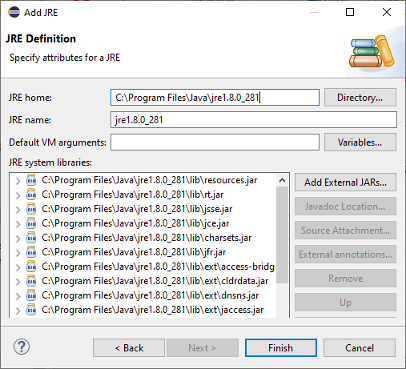
\includegraphics[]{images/EclipseJREDefinition}
\else
   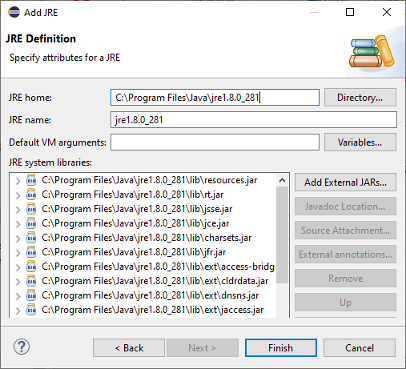
\includegraphics[width=0.6\textwidth]{images/EclipseJREDefinition}
\fi
\end{center}
\caption{Eclipse JRE Definition dialog.}
\label{JREDefinition:fig}
\end{figure}
\fi % end Windows

\item Click {\sf Finish}. Your Java JDK will now show up in the list
of installed JREs.
\ifWindows % begin Windows
Click on the left box to select it, as shown in
Figure \ref{InstalledJREs:fig} (ignore any warnings about Java 15
compatibility).
\fi % end Windows
\fi % end Not MacOS
\ifLinux % begin Linux
Click on the left box to select it; ignore any warnings about Java
15 compatibility.
\else % else NOT Linux
\begin{figure}[ht]
\begin{center}
\iflatexml
  \ifWindows
     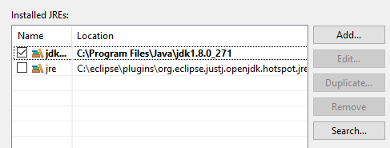
\includegraphics[]{images/EclipseInstalledJREs}
  \else
     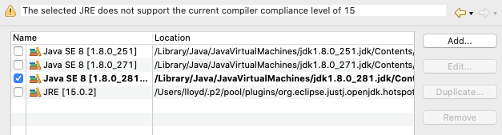
\includegraphics[]{images/EclipseInstalledJREsMacOS}
  \fi
\else
  \ifWindows
     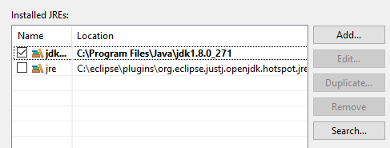
\includegraphics[width=0.6\textwidth]{images/EclipseInstalledJREs}
  \else
     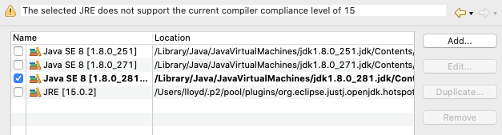
\includegraphics[width=0.8\textwidth]{images/EclipseInstalledJREsMacOS}
  \fi
\fi
\end{center}
\caption{Eclipse Installed JREs dialog.}
\label{InstalledJREs:fig}
\end{figure}
\fi % end NOT Linux

\item Finish by clicking the ``{\sf Apply and Close}'' button at the
bottom of the {\sf Preferences} dialog.

\end{enumerate}

\subsubsection{Preventing excess resource copying}

By default, ArtiSynth classes are placed in file tree located beneath
{\tt <ARTISYNTH\_HOME>\SEP classes} that is separate from the source
tree located beneath {\tt <ARTISYNTH\_HOME>\SEP src}.
That means that Eclipse will try to copy all non-Java files and
\directories{} from the source tree into the build tree. For ArtiSynth,
this is excessive, and results in many files being copied that don't
need to be, since ArtiSynth looks for resources in the source tree
anyway.

To prevent this copying:

\begin{enumerate}

\item Choose
\ifMacOS
``{\sf Eclipse > Preferences...}''.
\else
``{\sf Window > Preferences}''.
\fi

\item Select {\sf Java > Compiler > Building}.

\item Open {\sf Output folder}, and in the box entitled {\sf Filter resources},
  enter the single character `{\tt *}'.

\end{enumerate}

%\subsection{Importing ArtiSynth projects into Eclipse}
%
%ArtiSynth projects include the core distribution ({\tt
%artisynth\_core}), the open source models collection {\tt
%artisynth\_models} (which contains human anatomy models), as well as
%other model and code collections maintained by the ArtiSynth team and
%other users.
%
%If the project has already been downloaded or checked out from a
%repository, then it can be imported as an external project
%(Section \ref{importingExternalProjects}). Git repositories that
%contain Eclipse project files can be imported directly from within
%Eclipse (Section \ref{importingFromGit}), while those that contain the
%project files bundled up as a {\tt .zip} file can be cloned using
%Eclipse (Section \ref{importingFromGit}) and then imported as an
%external project after the project files have been unzipped into the
%top level \directory{}.

\subsection{Importing external projects}
\label{importingExternalProjects}

Let {\tt <PROJECT\_DIR>} denote the top-level \directory{}
of the project to be imported.
(In the case of {\tt artisynth\_core}, this will also be
\ArtHome[].) Assuming that {\tt <PROJECT\_DIR>} contains an Eclipse {\tt .project}
file, you can import it into Eclipse as follows:

\begin{enumerate}

\item From within Eclipse, choose ``{\sf File > Import ...}''.

\item An {\sf Import} dialog will appear. 
Select {\sf General > Existing Projects into Workspace} and click {\sf Next}.

\item An {\sf Import Projects} dialog will appear. 
In the field {\sf Select root directory}, enter (or browse to) the
{\it parent} \directory{} of {\tt <PROJECT\_DIR>}. The project
itself should now appear in the {\sf Projects} box (Figure
\ref{EclipseImportProjects:fig}). (If other projects are contained in the 
parent \directory{}, these will appear as well.)
Make sure that the
desired project is selected and then click {\sf Finish}.

\end{enumerate}

\begin{sideblock}
If Eclipse complains that {\sf "No projects are found to import"}, or
does not otherwise show the project as available for import,
then most likely the {\tt <PROJECT\_DIR>}
\directory{} does not contain a {\tt .project} file.
\end{sideblock}

\begin{figure}
\begin{center}
\iflatexml
  \ifWindows
     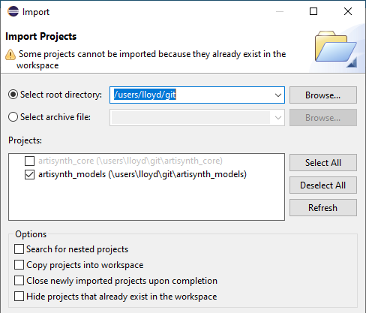
\includegraphics[]{images/EclipseImportProjects}
  \else
     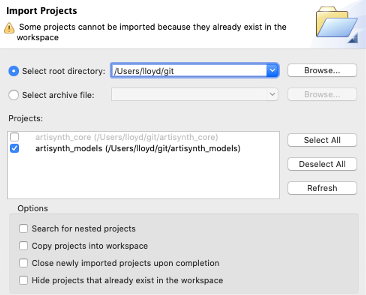
\includegraphics[]{images/EclipseImportProjectsMacOS}
  \fi
\else
  \ifWindows
     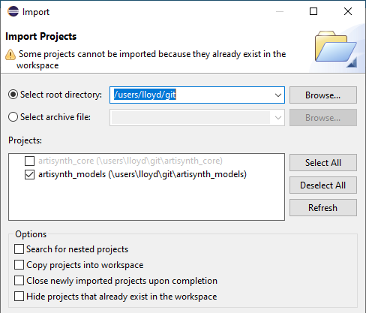
\includegraphics[width=0.7\textwidth]{images/EclipseImportProjects}
  \else
     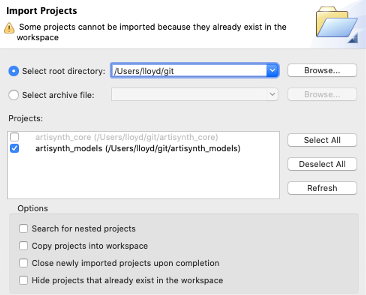
\includegraphics[width=0.7\textwidth]{images/EclipseImportProjectsMacOS}
  \fi
\fi   
\end{center}
\caption{Partial view of the Eclipse Import Projects dialog.}%
\label{EclipseImportProjects:fig}
\end{figure}

%\subsubsection{Importing projects from a remote Git repository}
%\label{importingFromGit}
%
%Some source repositories contain Eclipse project files in their
%repositories, and so can be imported directly into Eclipse using the
%repository's URL. The Eclipse project associated with ArtiSynth is
%called {\tt artisynth\_core}, while the models project is called {\tt
%artisynth\_models}.
%
%To import these directly:
%
%\begin{enumerate}
%
%\item If necessary, open a Java perspective by choosing {\sf Window >
%Open Perspective > Java}.
%
%\item Choose {\sf File > Import... > Git > Projects from Git}
%from the main menu.
%
%\item A {\sf Select Repository Source} dialog will appear. Choose
%{\sf Clone URI} and click {\sf Next}.
%
%\item A {\sf Source Git Repository} dialog will appear
%(Figure \ref{EclipseGitImport:fig}, left).  Under {\sf Location},
%enter the project URI in the {\sf URL} field.  The default URL for
%ArtiSynth is {\tt https://github.com/artisynth/artisynth\_core.git}. In
%some cases, such as when using an SSH URL, or accessing a project with
%restricted access, it may also be necessary to provide a user name and
%password in the {\sf Authentication} fields. (This will be your Gitlab
%or GitHub account information for repositories stored on those sites.)
%After entering the required information, click {\sf Next}.
%
%\item A {\sf Branch Selection} dialog may appear. If it does,
%make sure only the {\sf master} branch is selected, and then click {\sf Next}.
%
%\item A {\sf Local Destination} dialog will appear (Figure
%\ref{EclipseGitImport:fig}, right). In the {\sf Directory} field, enter
%the path of the local \directory{}, which will contain both the cloned
%repository and the working copy.  For ArtiSynth itself, this will also
%be the ArtiSynth home \directory{} (\ArtHome[]).  After
%entering the \directory{} information, click {\sf Next}.
%
%\item A {\sf Select a wizard ...} dialog will appear.
%Select {\sf Import existing Eclipse projects} and click {\sf Next}.
%
%\item An {\sf Import Projects} dialog will appear.
%Make sure project you wish to import is selected and click {\sf
%Finish}.
%
%\item In the case of ArtiSynth (i.e., {\tt artisynth\_core}), from {\it outside}
%Eclipse, download the Java and native libraries, as described in
%Section \ref{DownloadingLibraries}. Then refresh the project from
%within Eclipse (by selecting it in the {\sf Package Explorer} window
%and choosing {\sf Refresh} from the context menu. The project should
%now be able to compile.
%
%\end{enumerate}
%
%\begin{figure}[h]
%\begin{center}
%\begin{tabular}{cc}
%\iflatexml
%   \includegraphics{images/EclipseSourceGitRepositorySmall} &
%   \includegraphics{images/EclipseLocalDestinationSmall}
%\else
%   \includegraphics[width=0.45\textwidth]{images/EclipseSourceGitRepository} &
%   \includegraphics[width=0.45\textwidth]{images/EclipseLocalDestination}
%\fi   
%\end{tabular}
%\end{center}
%\caption{Eclipse dialogs for importing a Git repository.}%
%\label{EclipseGitImport:fig}
%\end{figure}
%
%\subsubsection{Cloning a project from a remote Git repository}
%\label{cloningFromGit}
%
%Some source repositories (such as {\tt artisynth\_research}) do not
%directly contain Eclipse project files in their repositories.
%Instead, the project files is contained inside an {\tt
%eclipseSettings.zip} file that must be extracted into the project root
%\directory{}. This is to prevent undesired local changes to the project
%settings from being propagated to all users.
%
%In this case, we proceed as follows:
%
%\begin{enumerate}
%
%\item Choose {\sf Window > Show View > Other ... > Git > Git Repositories} 
%from the main menu to open a {\sf Git Repositories} view window.
%
%\item Within the {\sf Git Repositories} window, choose the
%button (or pull down menu item) that says {\sf Clone a repository}.
%
%\item 
%A {\sf Source Git Repository} dialog will appear (Figure
%\ref{EclipseGitImport:fig}, left). Enter the URL for the
%repository. Also, if the repository has read access restrictions, it
%will generally be necessary to specify a user name and password in the
%{\sf Authentication} fields.  (This will be your Gitlab or GitHub
%account information for repositories stored on those sites.)  After
%entering the required information, click {\sf Next}.
%
%\item A {\sf Branch Selection} dialog may appear. Usually
%you want to select only the {\sf master} branch, and then click {\sf
%Next}.
%
%\item A {\sf Local Destination} dialog will appear (Figure
%\ref{EclipseGitImport:fig}, right). In the {\sf Directory} field, enter
%the path of the local \directory{}, which will contain both the cloned
%repository and the working copy. After entering the \directory{}
%information, click {\sf Finish}.
%
%\item Finally, from {\it outside} Eclipse, locate the file
%{\tt eclipseSettings.zip} in the project's top \directory{}, and then
%unzip this file directly into that \directory{} (not into a
%sub-\directory{}), so that {\tt .project} and {\tt .classpath} appear
%in the top \directory{}.
%\ifMacOS
%MacOS users are strongly encouraged to read  
%Section \ref{installingProjectFiles} for details on how to do this.
%\else
%For details, see Section \ref{installingProjectFiles}.
%\fi % end MacOS
%
%\end{enumerate}
%
%The project can now be imported into Eclipse by following the steps in
%Section \ref{importingExternalProjects}, using the project's
%parent \directory{} as the ``root directory''.
%
%\subsubsection{Installing project files}
%\label{installingProjectFiles}
%
%Some project repositories contain their eclipse project files bundled
%in the zip file {\tt eclipseSettings.zip}, instead of keeping them
%under direct repository control. This is to prevent unwanted local
%configuration changes from being propagated back into the repository.
%The project files need to be unzipped directly into the project
%\directory{} (not into a sub-\directory{}) to enable the project to be
%loaded into Eclipse.
%
%Let {\tt <PROJECT\_DIR>} denote the top-level project \directory{}.
%%
%\ifWindows
%On Windows, project files can be extracted from within the 
%file browser. Double click on {\tt eclipseSettings.zip}
%and extract the files into {\tt <PROJECT\_DIR>}.
%\else % not Windows 
%Project files can be extracted using the command line.
%Open a command shell, 
%switch to the {\tt <PROJECT\_DIR>} \directory{}, and run {\tt unzip}:
%\begin{verbatim}
%  > cd <PROJECT_ROOT>
%  > unzip eclipseSettings.zip
%\end{verbatim}
%\fi % end not Windows
%This will create the files {\tt .project} and {\tt .classpath}, along
%with the \directory{} {\tt .settings}, in {\tt <PROJECT\_DIR>}.  In
%the case of {\tt artisynth\_core}, it will also create the file {\tt
%ArtiSynth.launch} containing the default launch configuration.
%
%\begin{sideblock}
%Note: if unzip queries about overwriting {\tt .project}, answer [y]es.
%\end{sideblock}
%
%\ifMacOS
%\begin{sideblock}
%{\bf Attention MacOS users:}\\[0.5em]
%While it is possible to unzip files from the file browser by clicking
%on {\tt eclipseSettings.zip} and then extracting directly, the default
%zip utility on MacOS will create a new sub-folder called {\tt
%eclipseSettings} and will extract the files there.
%\emph{You do not want this!!}
%Some of the files are then labeled as ``hidden'' by MacOS, which will
%prevent you from moving them to the correct place manually. 
%Either extract the files using the command line as described
%above, or use a more standard application like {\sf 7-Zip} ({\sf 7zX} for OSX).
%\end{sideblock}
%\fi % end MacOS
%

\subsection{Configuring environment variables}
\label{EclipseEnvironmentVariables}

While it is generally {\it not} necessary to set environment variables
in Eclipse, it may be useful to do this on occasion to control certain
aspects of ArtiSynth's operation.  Directions on setting the
environment variables are given in
Section \ref{SettingEnvironmentVariables}, and descriptions of the
variables themselves may be found in
Section \ref{EnvironmentVariables}.

If any environment variables have already been set externally in
\SYSTEM{} (\environmentSectionRef), such that they are visible
to Eclipse at start-up, then they do {\it not} need to be set in the
launch configuration.

\ifNeedLibraryPath

\begin{sideblock}
{\bf Important:} At present, eclipse does not expand environment variables.
In all the variable settings described below, references to 
\ArtHome[]should be expanded (manually) to the path of the
ArtiSynth install \directory{}.
\end{sideblock}

\ifWindows
\begin{sideblock}
{\bf Note:} There is a bug in Eclipse 4.0+ on Windows where it will replace 
the system's native {\tt \%PATH\%} variable rather than appending to it.  
To correct this behavior, define \PATH{} as 
{\tt \$\{env\_var:path\};\$ARTISYNTH\_HOME\SEP lib\SEP \ARCH{}} 
\end{sideblock}
\fi % end Windows
\fi

\subsubsection {Setting environment variables}
\label{SettingEnvironmentVariables}

To set environment variables within Eclipse:

\begin{enumerate}

\item Open a java perspective if necessary by choosing
  {\sf Window > Open Perspective > Java}.

\item Select the ArtiSynth project in the {\sf Package Explorer} form.

\item Choose ``{\sf Run > Run Configurations...}'' to open the {\sf Run
  Configurations} window.

\item In the left panel, under {\sf Java Application}, select 
the launch configuration (the default is named {\sf ArtiSynth}).

\item In the right panel, select the {\sf Environment} tab.

\item To create a new environment variable, click the {\sf New} button and
  enter the name and value in the dialog box. 
%See Figure \ref{EclipseEnvVariables:fig}.

\item When finished, make sure that {\sf Append environment to native
  environment} is selected, and click {\sf Apply}.

\end{enumerate}

%\begin{figure}
%\begin{center}
%\iflatexml
%\includegraphics[]{images/EclipseEnvVariablesSmall}
%\else
%\includegraphics[width=5.0in]{images/EclipseEnvVariables}
%\fi
%\end{center}
%\caption{Setting environment variables within Eclipse.}%
%\label{EclipseEnvVariables:fig}
%\end{figure}

\subsection{Command line and JVM arguments}
\label{EclipseCommandArguments}

As described in Section \ref{CommandLineArguments}, the {\tt artisynth}
command accepts command line arguments. To invoke these when
running from Eclipse, it is necessary to set the desired arguments in
the launch configuration, as described below. 

Sometimes it may also be necessary to set JVM arguments, which control
the Java virtual machine running ArtiSynth.  An example of such an
argument is {\tt -Xmx}, which can be used to increase the maximum
amount of memory available to the application.  For example, {\tt
-Xmx6g} sets the maximum amount of memory to 6 gigabytes.

\subsubsection {Setting command line and JVM arguments}
\label{SettingCommandLineArguments}

To set command line arguments for your Eclipse application:

\begin{enumerate}

\item Open a java perspective if necessary by choosing
  {\sf Window > Open Perspective > Java}.

\item Select the ArtiSynth project in the {\sf Package Explorer} form.

\item Choose ``{\sf Run > Run Configurations...}'' to open the {\sf Run
  Configurations} window.

\item In the left panel, under {\sf Java Application}, select
the launch configuration (the default is named {\sf ArtiSynth}).

\item In the right panel, select the {\sf Arguments} tab.

\item Program arguments (which are passed directly to ArtiSynth)
should be specified in the {\sf Program arguments} box.  JVM arguments
should be specified in the {\sf VM arguments} box. See Figure
\ref{EclipseRunArguments:fig}.

\item When finished, click {\sf Close}.

\end{enumerate}

\begin{figure}
\begin{center}
\iflatexml
  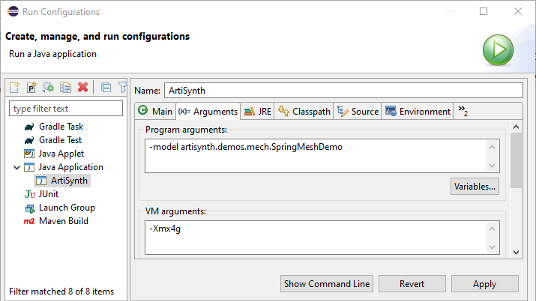
\includegraphics[]{images/EclipseLaunchConfig}
\else
  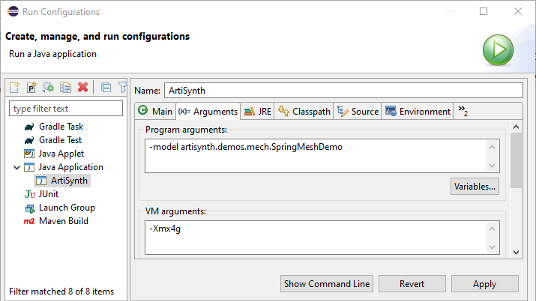
\includegraphics[width=6in]{images/EclipseLaunchConfig}
\fi
\end{center}
\caption{Editing command line and JVM arguments for a run configuration.}%
\label{EclipseRunArguments:fig}
\end{figure}

\subsection{Adding projects to the build path}
\label{AddingProjectsToBuildPath}

A project imported into Eclipse may depend on the packages and
libraries found in other projects to compile properly.  For example,
ArtiSynth applications which are external to {\tt artisynth\_core}
will nonetheless depend on {\tt artisynth\_core}. To ensure proper
compilation, project dependencies should be added to each dependent
project's build path.

\begin{enumerate}

\item Select the dependent project in the {\sf Package Explorer} form.

\item Right click and choose ``{\sf Build Path > Configure Build Path...}''

\item In the right panel, select the {\sf Projects} tab.

\item Click the {\sf Add} button, select the project dependencies,
      and click {\sf OK}

\item Click {\sf OK} in the Java Build Path panel

\end{enumerate}

\subsection{Adding projects to the ArtiSynth launch configuration}
\label{AddingProjectsToLaunch}

The classes of external projects can be made visible to ArtiSynth by
adding the projects themselves to the Classpath of the ArtiSynth launch
configuration.

\begin{enumerate}

\item From the main menu, choose ``{\sf Run > Run Configurations...}''
to open a {\sf Run Configurations} dialog.

\item In the left panel, under {\sf Java Application}, select your
ArtiSynth launch configuration (the default one is called {\sf
ArtiSynth}). This may already be selected when you open the panel.

\item In the right panel, select the {\sf Classpath} tab.

\item In the {\sf Classpath} window, select {\sf User Entries},
and then click the {\sf Add Projects} button.

\item In the {\sf Project Selection} dialog, select the external
projects that you wish to add. Generally, the boxes
``{\sf Add exported entries ...}'' and ``{\sf Add required projects ...}''
can be unchecked. Click {\sf OK}.

\item Close the {\sf Run Configurations} dialog.

\end{enumerate}

\section{Additional Information}

\subsection{Adding Directories to the System Path}
\label{SettingPath}

The system ``Path'' is a list of directories which the system searches
in order to find executables. Adding a directory to the path allows
executables contained in that directory to be called directly from a
\ifWindows
command window such as {\tt CMD}.
\else
terminal window.
\fi

\ifWindows

\subsubsection{Windows 10}

\begin{enumerate}

\item Open the {\sf Start} search, enter ``{\tt env}'', and choose
{\sf ``Edit the system environment variables''}.

\item Click on {\sf Environment Variables}.

\item Under {\sf User variables} (the top window), click on {\sf Path}
and click {\sf Edit}. If {\sf Path} does not exist, click {\sf New}.

\item In the {\sf Edit environment variable} dialog, click {\sf New}
and enter the full path name for each directory you wish to add.

\item Close each dialog by clicking {\sf OK}.

\end{enumerate}

\subsubsection{Windows 8 and earlier}

\begin{enumerate}

\item Right-click {\sf My Computer}, and then click {\sf Properties}.

\item Click the {\sf Advanced} tab.

\item Click {\sf Environment variables}.

\item In the top {\sf User variables} window, click on {\sf Path} and 
then {\sf Edit}. If {\sf Path} does not exist, click {\sf New}.

\item In the edit window, add the full path name for each new directory,
separated by semi-colons `{\tt ;}'.

\item Close each dialog by clicking {\sf OK}.

\end{enumerate}

For example, if ArtiSynth is installed at {\tt C:\BKS artisynth\BKS
artisynth\_core} and the desired {\tt JDK} is at {\tt C:\BKS Program
Files\BKS Java\BKS jdk1.8.0\_281}, then we can add the {\tt bin}
directories for both by setting the User path to
\begin{verbatim}
  C:\artisynth\artisynth_core\bin;C:\Program Files\Java\jdk1.8.0_281\bin
\end{verbatim}

\fi % end Windows

\ifWindows\else % not Windows

\ifMacOS
Since \SYSTEM{} is a Unix-based system, 
\else\ifLinux
On Linux,
\fi % end Linux
\fi % end not Windows
directories can be added to the path by appending them to the {\tt
PATH} environment variable, which is a list of directories separated
by colons `{\tt :}'. The most direct way to do this is to redefine
\PATH{} inside one of the initialization files for whichever
command line shell you are using.

Assume that your home folder is {\tt <HOMEDIR>}. Then for the {\tt
bash} shell, one can edit {\tt <HOMEDIR>/.bashrc} and insert a line of
the form
\begin{verbatim}
   export PATH=<DIR>:$PATH
\end{verbatim}
while for the {\tt csh} or {\tt tcsh} shells, one can edit {\tt
<HOMEDIR>/.cshrc} and insert a line of the form
\begin{verbatim}
   setenv PATH <DIR>":"$PATH
\end{verbatim}

\ifMacOS
On Mac OS X 10.8 and greater, directories can also be added to the
path by adding a text file containing the directories to {\tt
/etc/paths.d}.  In particular, we can create a file called {\tt
ArtiSynth} in {\tt /etc/paths.d} that contains the full path names of
the desired directories.

\begin{enumerate}

\item Open a terminal window

\item Use {\tt sudo} to create {\tt /etc/paths.d/ArtiSynth} with a plain
text editor. For example:
\begin{verbatim}
  sudo nano /etc/paths.d/ArtiSynth
\end{verbatim}

\item Add the full path name of each desired directory, one per line,
and save the file.

\item To test the revised \PATH{}, open a new terminal
window and enter the command: {\tt echo \$PATH}.

\end{enumerate}

\fi % end MacOS
\fi % end not Windows

\begin{sideblock}
Most most command windows and applications need to be restarted in
order to get them to notice changes to \PATH{}.
\end{sideblock}

\subsection{Environment variables}
\label{EnvironmentVariables}

This is a glossary of all the environment variables that are
associated with building or running ArtiSynth. Often, the system can
detect and set appropriate values for these automatically. In other
cases, as noted in the above documentation, it may be necessary or
desirable for the user to set them explicitly.

\begin{description}

\item[{\tt ARTISYNTH\_HOME}]\mbox{}
 
The path name of the ArtiSynth installation \directory{}.

%\item[ARTISYNTH\_PATH]\mbox{}
%
%A list of \directories{}, separated by \separatorDesc, which ArtiSynth
%uses to search for configuration files such as {\tt .artisyntInit} or
%{\tt demoModels.txt}.  A typical setting for {\tt ARTISYNTH\_PATH}
%consists of the current \directory{} (indicated by "{\tt .}"), the user's
%home \directory{}, and the ArtiSynth installation \directory{}. If {\tt
%ARTISYNTH\_PATH} is not defined explicitly in the user's environment,
%ArtiSynth assumes an implicit path consisting of the \directory{}
%sequence just described.

\item[{\tt CLASSPATH}]\mbox{}

A list of \directories{} and/or JAR files, separated by
\separatorDesc, which Java uses to locate its class files.

\item[\PATH{}]\mbox{}
 
A list of \directories{}, separated by \separatorDesc, which the
operating system uses to locate executable programs and
applications. Placing \ArtHome[\SEP bin] in \PATH{} (as
described in Section \ref{SettingPath}) will allow you to run {\tt
artisynth} and related commands directly from a command window.

\ifNeedLibraryPath
\ifWindows\else % not Windows 
\item[\LIBRARYPATH{}]\mbox{}

A list of \directories{}, separated by colons
":", which the operating system searches in order to find shared libraries.
Should be set to include \ArtHome[\SEP lib\SEP \ARCH{}].
\fi % end not Windows
\fi % end NeedLibraryPath

\item[{\tt OMP\_NUM\_THREADS}]\mbox{}
 
Specifies the maximum number of processor cores that are available for
multicore execution. If not set, the system uses the
maximum number of cores available. Users can also set this number from
within ArtiSynth by setting the configuration property {\sf
numSolverThreads}, either for the current session by choosing {\sf
``Settings > Interaction ...''} from the main menu, or for all sessions by
choosing {\sf ``Settings > Preferences ... > Interaction''}.

\end{description}

%JYTHON\_HOME::
%If Jython is installed on the system, should be set to the name of the
%Jython installation \directory{}.

Note that settings for most of the above can be derived from the value
of {\tt ARTISYNTH\_HOME}.

\ifWindows
\subsubsection{Setting environment variables}
\label{settingWindowsVariables}

On Windows, a user can view, set, or change environment variables via
the following steps:

{\bf Windows 10:}

\begin{enumerate}

\item Open the {\sf Start} search, enter ``{\tt env}'', and choose
{\sf ``Edit the system environment variables''}.
\item Click on {\sf Environment Variables}.
\item Choose one of the following options:

\begin{itemize}
\item Click {\sf New} to add a new variable name and value.
\item Click an existing variable, and then {\sf Edit} to change its name or value.
\item Click an existing variable, and then {\sf Delete} to remove it.
\end{itemize}

\item Close each dialog by clicking {\sf OK}.

\end{enumerate}

{\bf Windows 8 and earlier:}

\begin{enumerate}

\item Right-click {\sf My Computer}, and then click {\sf Properties}.
\item Click the {\sf Advanced} tab.
\item Click {\sf Environment variables}.
\item Choose one of the following options:

\begin{itemize}
\item Click {\sf New} to add a new variable name and value.
\item Click an existing variable, and then {\sf Edit} to change its name or value.
\item Click an existing variable, and then {\sf Delete} to remove it.
\end{itemize}

\item Close each dialog by clicking {\sf OK}.

\end{enumerate}

Variable settings can reference other environment variables by
surrounding them with percent signs, as in {\tt \%VAR\_NAME\%}.  For
example, suppose you already have an environment variable {\tt HOME} that
gives the location of your home \directory{}, and your ArtiSynth
distribution is located in {\tt packages\SEP artisynth\_core} relative to your
home \directory{}. Then the environment variable {\tt ARTISYNTH\_HOME} can be
specified as

\begin{verbatim}
  %HOME%\packages\artisynth_core
\end{verbatim}

\subsubsection{Typical environment settings}
\label{TypicalEnvironment}

Typical settings for the environment variables described above might
look like this:

\begin{lstlisting}[]
ARTISYNTH_HOME c:\users\joe\artisynth_core
CLASSPATH %ARTISYNTH_HOME%\classes;%ARTISYNTH_HOME%\lib\*
PATH %ARTISYNTH_HOME%\bin;%PATH%
\end{lstlisting}

\subsubsection{GitBash environment settings}
\label{GitBashEnvironmentSettings}

When using {\tt GitBash} (Section \ref{GitForWindows}), it is
possible to set environment variables in a {\tt .bashrc} file located
in the user's home \directory{}. The file entries corresponding
to the settings of Section \ref{TypicalEnvironment}
would look like this:

\begin{lstlisting}[]
# set ARTISYNTH_HOME to the appropriate location ...
export ARTISYNTH_HOME=C:/users/joe/artisynth_core
# Windows file notation is needed for CLASSPATH:
AH="C:\users\joe\/artisynth_core"
export CLASSPATH="$AH\classes;$AH\lib\*"
export PATH=$ARTISYNTH_HOME/bin:$PATH
\end{lstlisting}

Note that the {\tt CLASSPATH} environment variable must be set using a
Windows format, with backslash ('\BKS') to separate files and
semicolon (';') to separate path entries. This requirement is
imposed by the Java compiler.
\fi % end Windows

\ifWindows\else % not Windows 
\subsubsection{Example environment set up for {\tt bash}}
\label{BashEnvironmentSetup}

If you are using {\tt bash} as your shell, then the environment can be
configured by placing a block of commands similar to the following in
one of your {\tt bash} initialization files (typically {\tt
\textasciitilde/.bashrc}), located in your home \directory{}:

\begin{lstlisting}[]
# set ARTISYNTH_HOME to the appropriate location ...
export ARTISYNTH_HOME=$HOME/artisynth_core
export CLASSPATH="$ARTISYNTH_HOME/classes:$ARTISYNTH_HOME/lib/*"
export PATH="$ARTISYNTH_HOME/bin:$PATH"
\end{lstlisting}

Be sure to set {\tt ARTISYNTH\_HOME} to the proper location of your
ArtiSynth installation \directory{}.

These environment variables will be passed on to any program which you
run from the shell (such as {\tt artisynth} or {\tt eclipse}).
\ifMacOS
However, they will {\bf not} be passed on to programs (such as eclipse)
which you launch from the dock.
\fi

Alternatively, you can source the script {\tt setup.bash}, located in
the installation \directory{}:

\begin{verbatim}
 > source setup.bash
\end{verbatim}

This will determine the system type automatically and set the
environment variables accordingly, with {\tt ARTISYNTH\_HOME} set to the
current \directory{} from which the script is called.

\subsubsection{Example environment setup for {\tt csh} or {\tt tcsh}}
\label{CshEnvironmentSetup}

If you are using {\tt csh} or {\tt tcsh} as your shell, then the
environment can be configured by placing a block of commands similar
to the following in your {\tt .cshrc} file, located in your home
\directory{}:

\ifLinux
\begin{lstlisting}[]
# set ARTISYNTH_HOME to the appropriate location ...
setenv ARTISYNTH_HOME $HOME/artisynth_core
setenv CLASSPATH "$ARTISYNTH_HOME/classes:$ARTISYNTH_HOME/lib/*:$CLASSPATH"
setenv PATH $ARTISYNTH_HOME/bin":"$PATH
\end{lstlisting}
\else\ifMacOS
\begin{lstlisting}[]
# set ARTISYNTH_HOME to the appropriate location ...
setenv ARTISYNTH_HOME $HOME/artisynth_core
setenv CLASSPATH "$ARTISYNTH_HOME/classes:$ARTISYNTH_HOME/lib/*:$CLASSPATH"
setenv PATH $ARTISYNTH_HOME/bin":"$PATH
\end{lstlisting}
\fi % end MacOS
\fi % end not Linux

These environment variables will be passed on to any program which you
run from the shell (such as {\tt artisynth} or {\tt eclipse}).
\ifMacOS
However, they will {\bf not} be passed on to programs (such as eclipse)
which you launch from the dock.
\fi

Alternatively, you can source the script {\tt setup.csh}, located in
the installation \directory{}:

\begin{verbatim}
 > source setup.csh
\end{verbatim}

This will determine the system type automatically and set the
environment variables accordingly, with {\tt ARTISYNTH\_HOME} set to the
current \directory{} from which the script is called.
\fi % end not Windows

\subsection{ArtiSynth Libraries}

ArtiSynth uses a set of libraries located under
\ArtHome[\SEP lib].  These include a number of JAR
files, plus native libraries located in architecture-specific
sub-\directories{} ({\tt \ARCH{}} for \FULLSYSTEM{} systems).

As described in Section \ref{GitHubInstall}, these libraries
need to be downloaded automatically if the system is obtained from the
GitHub repository. The required libraries are listed in the file
\ArtHome[\SEP lib\SEP LIBRARIES]. This file is checked
into the repository, so that the system can always determine what
libraries are needed for a particular checkout version.

Occasionally the libraries are changed or upgraded
(Section \ref{UpdatingArtiSynth}).  If you run ArtiSynth with the {\tt
-updateLibs} command line option, the program will ensure that not
only are all the required libraries present, but that they also match
the latest versions on the ArtiSynth server.

\subsection{The EXTCLASSPATH File}
\label{EXTCLASSPATHFile}

The {\tt EXTCLASSPATH} file is stored in the user configuration folder
(Section \ref{UserConfigFolder:sec}) and contains the entries for the
external class path (Section \ref{ExternalClasspath:sec}).  It is
usually edited within ArtiSynth by selecting {\sf ``External classpath
...''} from the {\sf Settings} menu but can also be edited directly.
Each file entry describes a class \directory{} or JAR file needed to
run models external to the core ArtiSynth package.  Entries are
usually placed one per line, but multiple entries can be made on the
same line if separated by \separatorDesc{}.

The syntax rules for {\tt EXTCLASSPATH} are:

\begin{enumerate}

\item Entries on the same line should be separated
\separatorDesc{}.

\item The `{\tt \#}' character comments out all remaining characters
to the end of line.

\item The `{\tt \$}' character can be used to expand environment variables.

\item Any spaces present {\it will} be included in the entry name.

\end{enumerate}

An example {\tt EXTCLASSPATH} might look like this:

\ifWindows
\begin{verbatim}
C:\research\artisynth_models\classes
C:\research\models\special.jar
$HOME\projects\crazy\classes
\end{verbatim}
\else % not Windows 
\begin{verbatim}
/research/artisynth_models/classes
/research/models/special.jar
$HOME/projects/crazy/classes
\end{verbatim}
\fi % end not Windows

\subsection{Quick Git Summary}
\label{GitSummary}

Git is a distributed source control management (SCM) system that is
widely used in the software industry.  A full discussion of Git is
beyond the scope of this document, but a large literature is available
online. Generally, when you {\it clone} a Git repository, you create a
local copy of that repository on your machine, along with a checked
out working \directory{} containing the most recent version of the code
(which is referred to as the HEAD).

Unlike client/server SCMs, Git is distributed, with users maintaining
their own private copies of a repository. This allows a great deal of
flexibility in usage, but also adds an extra ``layer'' to the
workflow: when you ``checkout'' from a repository or ``commit'' to it,
you do so with respect to your own {\it local} copy of that
repository, {\it not} the original ({\it origin}) repository from
which you performed the original clone. The process of merging in
changes from the origin to the local repository is known as
``pulling'', while committing changes from the local repository back
to the origin is known as ``pushing''.

There is also another layer of interaction when you commit changes to
the local repository: you first {\it add} them to a staging area
(also known as the ``index''), and then commit them using the {\tt commit}
command.

A very simple workflow for a typical ArtiSynth user is summarized
below. The actions are described in command-line form, but the same
commands can generally be issued through Eclipse or other
interfaces. First, clone the most recent version of the ArtiSynth
repository on GitHub:

\begin{verbatim}
  git clone https://github.com/artisynth/artisynth_core.git [<dir>]
\end{verbatim}

This will create a local copy of the GitHub repository, along with a
checked out ``working copy'', in the \directory{} specified by {\tt
<dir>}, or in {\tt artisynth\_core} if {\tt <dir>} is
omitted.  The repository itself will be located in a sub-\directory{}
called {\tt .git}.

Other Git repositories can be cloned in a similar manner.  If the
repository has read access restrictions, then when performing a checkout it
may also be necessary to specify a user name for which the repository
has granted read access. This is typically done by embedding the user
name in the URL, as in (for example):

{\tt https://user@host.xz/path/to/repo.git}

Later, to fetch the latest updates from the GitHub repository and
merge them into your working copy, from within the working copy
\directory{} you can do
\begin{verbatim}
  git pull
\end{verbatim}

If you make changes to some files in your working copy and wish to
commit these to your local repository, you first {\it add} (or remove
them) from the staging area using commands such as:
\begin{verbatim}
  git add <fileName>    # add a new (or modified) file
  git add *             # add all files
  git rm <fileName>     # remove a file
\end{verbatim}
and then commit them to your local repository using
\begin{verbatim}
  git commit -m "commit message"
\end{verbatim}
Note that you can also add modified files and commit them using the single
command
\begin{verbatim}
  git commit -m -a "commit message"
\end{verbatim}

To see the current status of the files in your working copy
and the staging area, use the command
\begin{verbatim}
  git status
\end{verbatim}
and to see the commit history for particular files or \directories{},
use 
\begin{verbatim}
  git log [ <filename> ... ]
\end{verbatim}

Finally, to push your changes back to the GitHub repository (assuming
you have permission do so), you would do so using the command
\begin{verbatim}
  git push origin master
\end{verbatim}

Note that the above commands all have various options not mentioned.
There are also numerous topics that haven't been discussed, including
the creation and merging of branches, but there are many useful online
resources that describe these in detail. Some current references
include
\begin{verbatim}
   https://git-scm.com/docs
   http://rogerdudler.github.io/git-guide
\end{verbatim}


\end{document}

